\documentclass[10pt,a4paper]{article}
\usepackage[utf8]{inputenc}
\usepackage[spanish]{babel}
\usepackage{amsmath}
\usepackage{amsfonts}
\usepackage{amssymb}
\usepackage{graphics}
\usepackage{graphicx}
\usepackage{xcolor}
\usepackage{listings}
\usepackage{csvsimple}
\usepackage{caption}
\usepackage{subcaption}
\usepackage[left=2cm,right=2cm,top=2cm,bottom=2cm]{geometry}

\renewcommand*\contentsname{Índice} %Nombre del indice

\begin{document}
\lstset{
	basicstyle=\footnotesize,
	extendedchars=true,
	literate={á}{{\'a}}1 {ã}{{\~a}}1 {é}{{\'e}}1 {ú}{{\'u}}1 {ó}{{\'o}}1,
	backgroundcolor=\color{black!5}
	}
	
\begin{titlepage}
	\centering
	{
\includegraphics[scale=0.5]{Logo_UGR.png}\par}
	\vspace{1cm}
	{\bfseries\Large Escuela T\'ecnica Superior de Ingeniería Informática y Telecomunicaciones \par}
	\vspace{2.5cm}
	{\scshape\Huge Pr\'actica 1: An\'alisis de eficiencia de algoritmos \par}
	\vspace{3cm}
	{\itshape\Large Doble Grado Ingeniería Informática y Matemáticas}
	\vfill
	{\Large Autores: \par}
	{\Large Jose Alberto Hoces Castro\par}
	{\Large Javier Gómez López \par}
	{\Large Moya Mart\'in Castaño \par}
	\vfill
	{\Large Marzo 2022 \par}
\end{titlepage}

\thispagestyle{empty}
\null
\vfill

%%Información sobre la licencia
\parbox[t]{\textwidth}{
  
\includegraphics[scale=0.05]{by-nc-sa.png}\\[4pt]
  \raggedright % Texto alineado a la izquierda
  \sffamily\large
  {\Large Este trabajo se distribuye bajo una licencia CC BY-NC-SA 4.0.}\\[4pt]
  Eres libre de distribuir y adaptar el material siempre que reconozcas a los\\
  autores originales del documento, no lo utilices para fines comerciales\\
  y lo distribuyas bajo la misma licencia.\\[4pt]
  \texttt{creativecommons.org/licenses/by-nc-sa/4.0/}
}

\newpage

\tableofcontents

\newpage
\section{Introducción}

A modo de notación, destacamos las siguientes equivalencias:
\begin{itemize}
	\item \textit{Ordenador de Javier} \(\longrightarrow\) i7-6700 3.40 GHz.
	\item \textit{Ordenador de Jose Alberto} \(\longrightarrow\) i5-1035G1 1.00 GHz.
	\item \textit{Ordenador de Manuel} \(\longrightarrow\)i5-7200 2.5GHz.
\end{itemize}

Esta primera práctica, \textbf{Práctica 1}, consiste en el análisis de eficiencia de algoritmos, consiste en tres partes distintas:
\begin{itemize}
	\item \textbf{Análisis de la eficiencia teórica:} estudio de la complejidad teórica del algoritmos (Mejor caso, peor caso y caso promedio).
	\item \textbf{Análisis de la eficiencia empírica:} ejecución y medición de tiempos de ejecución de los algoritmos estudiados.
	\item \textbf{Análisis de la eficiencia híbrida:} obtención de las constantes ocultas
\end{itemize}

A continuación, se explican en más profundidad dichas partes.

\subsection{Análisis de la eficiencia teórica}

El análisis de la \textbf{eficiencia teórica} consiste en analizar el tiempo de ejecución de los algoritmos dados para encontrar el peor de los casos, es decir, en qué clase de funciones en notación \(\mathcal{O}\) grande se encuentran. Para ello, hemos utilizado las técnicas de análisis de algoritmos vistas en clase y en la asignatura \textit{Estructura de Computadores}.

\subsection{Análisis de la eficiencia empírica}

Para el análisis de la \textbf{eficiencia empírica}, hemos ejecutado los algoritmos en cada uno de nuestros equipos bajo las mismas normas y condiciones, hemos medido el tiempo de ejecución de dichos algoritmos con la biblioteca \texttt{<chrono>}, basándonos en la siguiente estructura del código:

\begin{lstlisting}
#include <chrono>
...

high_resolution_clock::time_point tantes, tdespues;
duration <double> transcurrido;
..

tantes = high_resolution_clock::now();
//Sentencia o programa a medir
tdepues = high_resolution_clock::now();
transcurrido = duration_cast<duration<double>>(tdespues-tantes);
\end{lstlisting}

Además, para automatizar el proceso de ejecución de los algoritmos, hemos usado la siguiente estructura para generar nuestros scripts:
\begin{lstlisting}[language=bash]
i = #valor de la primera iteracion

while [ $i -le #valor ultima iteracion ]
do
./programa_a_ejecutar $i >> salida.dat
i=$[i+#salto entre valores para conseguir 26 puntos]
done
\end{lstlisting}

Hemos ejecutado cada algoritmo 15 veces en cada uno de los tamaños que han sido probados, y hemos hecho la media de ellos para reducir perturbaciones que puedan ocurrir de manera aleatoria y que nos lleven al mejor o peor caso, obteniendo de esta forma el caso promedio. 

Cabe destacar que para \textit{seleccion} e \textit{insercion} hemos además ejecutado dos programas adicionales para obtener el mejor y peor caso de estos, pero este hecho lo detallaremos más adelante. \\

\subsection{Análisis de la eficiencia híbrida}
Para el análisis de la eficiencia híbrida, hemos tomado los datos de cada uno de los alumnos del grupo y hemos hallado la \(K\) (constante oculta). Para ello, hemos usado gnuplot. \\

Lo primero que hacemos es definar la función a la que queremos ajustar los datos. Tenemos que tener en cuenta el análisis teórico que hemos realizado previamente para saber cuál va a ser la forma de esta función. Podemos definir esta función en gnuplot mediante el siguiente comando (ejemplo para \(\mathcal{O}(n^2)\)):
\begin{lstlisting}[language=bash]
gnuplot> f(x) = a0*x*x+a1*x+a2
\end{lstlisting}

El siguiente paso es indicarle a gnuplot que haga la regresión usando el método de mínimos cuadrados:
\begin{lstlisting}
gnuplot> fit f(x) 'salida.dat' via a0,a1,a2
\end{lstlisting}
donde \texttt{'salida.dat'} es nuestro dataset. 

La parte que más nos interesa es la parte donde pone \texttt{Final set of parameters}, pues ahí están nuestros coeficientes junto con la bondad del ajuste realizado.

\section{Desarrollo}

A continuación, realizaremos el estudio individual de cada algortimo, como se ha descrito anteriormente.

\subsection{Inserción}
\scalebox{0.75}{
\lstinputlisting[language=C++]{./Codes/insercion.cpp}
}

\subsubsection{Eficiencia teórica}
Tal y como se ha indicado en los comentarios del código, todas las operaciones de asignación son \(\mathcal{O}(1)\). Estas, a su vez, se incluyen en un bucle \texttt{for} y un bucle \texttt{while}, que están anidados, y que por ser cada uno \(\mathcal{O}(n)\), multiplicamos lor órdenes de ambos como se vio en teoría, obteniendo que la función \texttt{static void insercion\_lims} es \(\mathcal{O}(n^2)\), es decir,
\[
T(n) \in \mathcal{O}(n^2)
\]
donde \(T(n)\) es la función que expresa el tiempo de ejecución del algoritmo.

\subsubsection{Eficiencia empírica}
Tras ejecutar el algortimo en un rango de 10000 a 200000 elementos, con saltos de 7600 unidades por ejecución, obtenemos los siguientes resultados:

\begin{table}[h!]
	\centering
	\footnotesize
	\scalebox{0.75}{
		\begin{tabular}{|c|c|}
			\hline
			\multicolumn{2}{|c|}{\textsf{Ordenador Javier}}
			\\\hline
			\bfseries Elementos (n) & \bfseries Tiempo (s)
			\csvreader{./data/Javi5454/salida_insercion.csv}{}
			{\\\hline\csvcoli&\csvcolii}
			\\\hline
		\end{tabular}
	}
	\hspace{2cm}
	\scalebox{0.75}{
		\begin{tabular}{|c|c|}
			\hline
			\multicolumn{2}{|c|}{\textsf{Ordenador José Alberto}}
			\\\hline
			\bfseries Elementos (n) & \bfseries Tiempo (s)
			\csvreader{./data/Jota/salida_insercion.csv}{}
			{\\\hline\csvcoli&\csvcolii}
			\\\hline
		\end{tabular}
	}
	\hspace{2cm}
	\scalebox{0.75}{
		\begin{tabular}{|c|c|}
			\hline
			\multicolumn{2}{|c|}{\textsf{Ordenador Manuel}}
			\\\hline
			\bfseries Elementos (n) & \bfseries Tiempo (s)
			\csvreader{./data/Moya/salida_insercion.csv}{}
			{\\\hline\csvcoli&\csvcolii}
			\\\hline
		\end{tabular}
	}
	\caption{Experiencia empírica de algoritmo de Inserción sin optimizar}
\end{table}

En este caso, al igual que en el resto de algoritmos, percibimos un poco de diferencia entre los tiempos de ejecución, debido a las diferentes circunstancias de cada integrante del grupo, pues poseemos dispositivos con distinto potencial.

\subsubsection{Eficiencia híbrida}
El estudio de la eficiencia híbrida consiste en hallar la expresión de las funciones que representan el tiempo de ejecución a partir de un tamaño dado. Usando los datasets del anterior apartado, hemos usado gnuplot para graficar los 26 puntos obtenidos junto con su función de ajuste. A continuación mostramos la gráfica con los ajustes de cada uno de los integrantes:

\begin{figure}[h!]
	\centering
	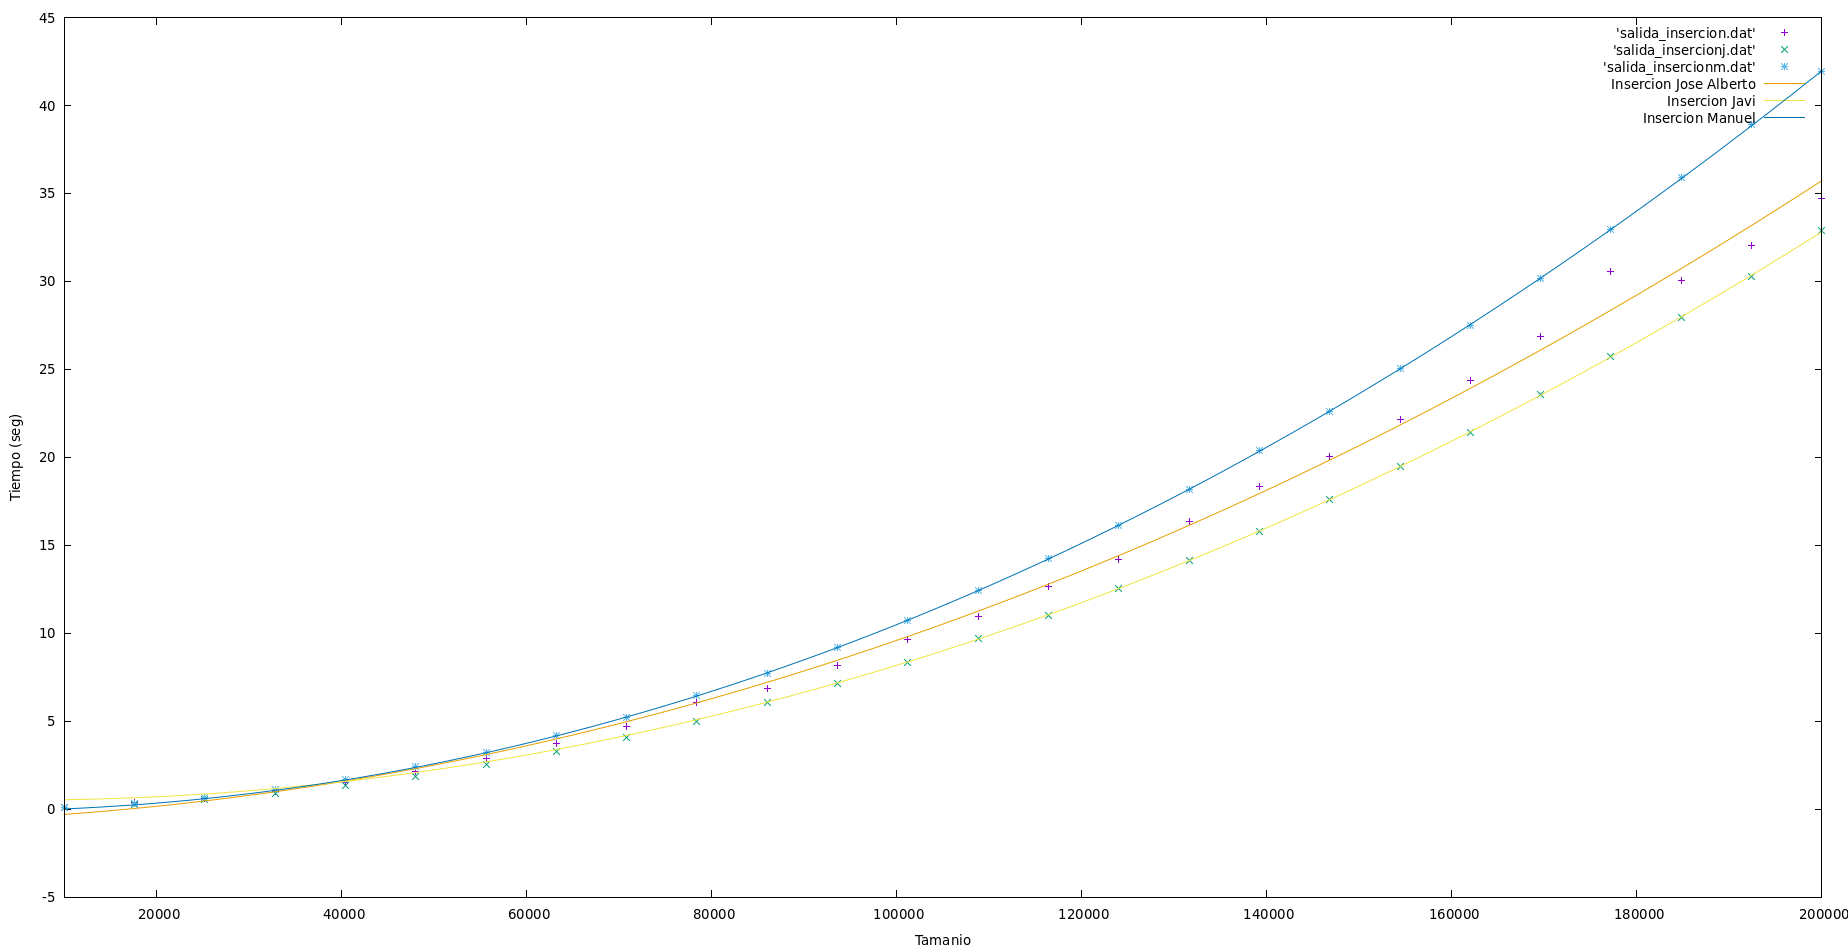
\includegraphics[scale=0.16]{../../Images/Insercion_combinados.png}
	\caption{Gráfica con los tiempos de ejecución del \\algoritmo de Inserción}
\end{figure}

Y las constantes ocultas son:

\begin{itemize}
	\item Ordenador Javier \(\rightarrow T_1(n) = 8.49924 \cdot 10^{-10} x^2 - 8.57879 \cdot 10^{-6} x + 0.546581\).
	\item Ordenador José Alberto \(\rightarrow T_2(n) = 7.96341 \cdot 10^{-10} x^2 + 2.23563 \cdot 10^{-5} x - 0.592279\).
	\item Ordenador Manuel \(\rightarrow T_3(n) = 1.04394 \cdot 10^{-9} x^2 + 1.58593 \cdot 10^{-6} x - 0.0969414\).
\end{itemize}

Para terminar nuestro análisis de este algoritmo, terminaremos de confirmar que el ajuste cuadrático es el óptimo viendo la varianza residual que nos ha proporcionado gnuplot:

\begin{itemize}
	\item \(T_1(n) \longrightarrow Var.res = 0.00162352\)
	\item \(T_2(n) \longrightarrow Var.res = 0.0050675\)
	\item \(T_3(n) \longrightarrow Var.res = 0.00161535\)
\end{itemize}

Como todas son muy próximas a 0, podemos asegurar que el ajuste es muy bueno.

\subsection{Selección}
\lstinputlisting[language=C++]{./Codes/seleccion.cpp}

\subsubsection{Eficiencia teórica}
Tal y como se ha indicado en los comentarios del código, todas las operaciones de asignación son \(\mathcal{O}(1)\). Estas, a su vez, se incluyen en dos bucles \texttt{for} que están anidados, que por ser cada uno \(\mathcal{O}(n)\), multiplicamos lor órdenes de ambos como se vio en teoría, obteniendo que la función \texttt{static void seleccion\_lims} es \(\mathcal{O}(n^2)\), es decir,
\[
T(n) \in \mathcal{O}(n^2)
\]
donde \(T(n)\) es la función que expresa el tiempo de ejecución del algoritmo.

\subsubsection{Eficiencia empírica}
Tras ejecutar el algortimo en un rango de 10000 a 200000 elementos, con saltos de 7600 unidades por ejecución, obtenemos los siguientes resultados:

\begin{table}[h!]
	\centering
	\footnotesize
	\scalebox{0.75}{
		\begin{tabular}{|c|c|}
			\hline
			\multicolumn{2}{|c|}{\textsf{Ordenador Javier}}
			\\\hline
			\bfseries Elementos (n) & \bfseries Tiempo (s)
			\csvreader{./data/Javi5454/salida_seleccion.csv}{}
			{\\\hline\csvcoli&\csvcolii}
			\\\hline
		\end{tabular}
	}
	\hspace{2cm}
	\scalebox{0.75}{
		\begin{tabular}{|c|c|}
			\hline
			\multicolumn{2}{|c|}{\textsf{Ordenador José Alberto}}
			\\\hline
			\bfseries Elementos (n) & \bfseries Tiempo (s)
			\csvreader{./data/Jota/salida_seleccion.csv}{}
			{\\\hline\csvcoli&\csvcolii}
			\\\hline
		\end{tabular}
	}
	\hspace{2cm}
	\scalebox{0.75}{
		\begin{tabular}{|c|c|}
			\hline
			\multicolumn{2}{|c|}{\textsf{Ordenador Manuel}}
			\\\hline
			\bfseries Elementos (n) & \bfseries Tiempo (s)
			\csvreader{./data/Moya/salida_seleccion.csv}{}
			{\\\hline\csvcoli&\csvcolii}
			\\\hline
		\end{tabular}
	}
	\caption{Experiencia empírica de algoritmo de Selección sin optimizar}
\end{table}

Observamos pequeñas diferencias en los tiempos de ejecución de cada uno de los ordenadores de los integrantes del grupo, y esto se debe a las condiciones específicas de cada uno de nuestros dispositivos y las prestaciones que estos tienen.

\subsubsection{Eficiencia híbrida}

Gracias al estudio de la eficiencia híbrida veremos que el ajuste teórico hecho hace dos subapartados es el correcto. Para ello, hemos tomado los datasets recién mostrados y hemos generado una gráfica en la que se representan los 26 tiempos obtenidos en función de los tamaños que hemos probado. Gnuplot nos ha facilitado esta gráfica junto con las constantes específicas asociadas a cada uno de nuestro, así como las varianzas residuales:

\begin{figure}[h!]
	\centering
	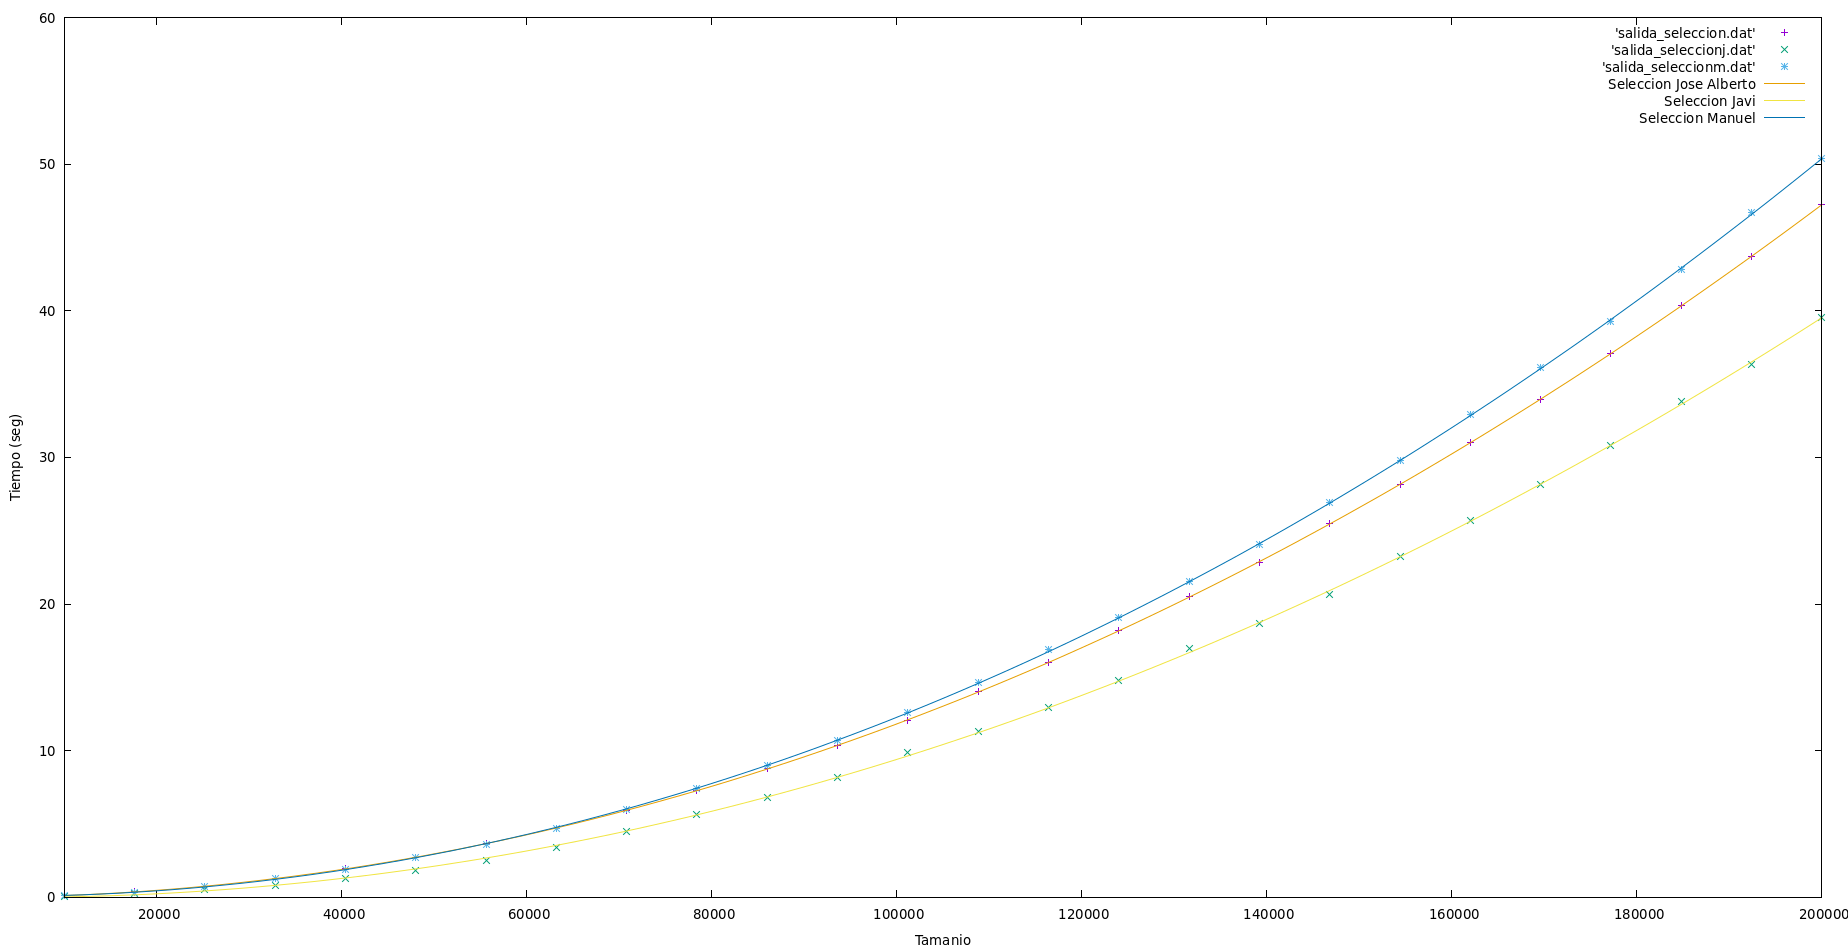
\includegraphics[scale=0.15]{../../Images/Seleccion_combinados.png}
	\caption{Gráfica con los tiempos de ejecución del \\algoritmo de Selección}
\end{figure}

Y las constantes ocultas son:
\begin{itemize}
	\item Ordenador Javier \(\rightarrow T_1(n) = 1.0371 \cdot 10^{-9} x^2 + -9.86278 \cdot 10^{-6} x +0.0216418\).
	\item Ordenador José Alberto \(\rightarrow T_2(n) = 1.17905 \cdot 10^{-9} x^2 + 3.97249 \cdot 10^{-7} x - 0.00421685\).
	\item Ordenador Manuel \(\rightarrow T_3(n) = 1.29484 \cdot 10^{-9} x^2 - 7.43377 \cdot 10^{-6} x + 0.0733569\).
\end{itemize}

Y para terminar de confirmar que nuestro ajuste es el correcto, podemos ver el valor de la varianza residual en cada caso:

\begin{itemize}
	\item \(T_1(n) \longrightarrow Var.res = 0.0164518\)
	\item \(T_2(n) \longrightarrow Var.res = 0.000537586\)
	\item \(T_3(n) \longrightarrow Var.res = 0.00387134\)
\end{itemize}

Vemos que en todos los casos el ajuste cuadrático nos da varianzas muy próximas a 0, por lo que es un ajuste óptimo.

\subsection{Quicksort}
\lstinputlisting[language=C++]{./Codes/quicksort.cpp}
\subsubsection{Eficiencia teórica}
Tras un análisis rápido del código podemos ver como quicksort es una función recursiva que divide el vector a ordenar de tamaño n en dos vectores de tamaño aproximadamente \(\frac{n}{2}\). Obviaremos la parte de la función en la que por debajo del umbral se ejecuta la función \texttt{insercion\_lims} ya que no es de nuestro interés en el análisis. Luego es fácil ver que la ecuación recurrente asociada es la siguiente ya que la función \texttt{dividir\_qs} es evidentemente \(\mathcal{O}(n)\):
\\
\(T(n) = 2T(\frac{n}{2}) + n \)
\\
cuya solución sabemos que es por los resultados vistos en clase 
\\
\(T(n) = c1 \cdot n + c2 \cdot n\log(n) donde c1, c2 \in \mathbb{R^+} \)
\\
Por tanto es claro que ocurre que:
\[
T(n) \in \mathcal{O}(n\log(n))
\]
donde \(T(n)\) es la función que expresa el tiempo de ejecución del algoritmo.

\subsubsection{Eficiencia empírica}
Tras ejecutar el algortimo en un rango de 100000 a 2000000 elementos, con saltos de 76000 unidades por ejecución, obtenemos los siguientes resultados:

\begin{table}[h!]
	\centering
	\footnotesize
	\scalebox{0.75}{
		\begin{tabular}{|c|c|}
			\hline
			\multicolumn{2}{|c|}{\textsf{Ordenador Javier}}
			\\\hline
			\bfseries Elementos (n) & \bfseries Tiempo (s)
			\csvreader{./data/Javi5454/salida_quicksort.csv}{}
			{\\\hline\csvcoli&\csvcolii}
			\\\hline
		\end{tabular}
	}
	\hspace{2cm}
	\scalebox{0.75}{
		\begin{tabular}{|c|c|}
			\hline
			\multicolumn{2}{|c|}{\textsf{Ordenador José Alberto}}
			\\\hline
			\bfseries Elementos (n) & \bfseries Tiempo (s)
			\csvreader{./data/Jota/salida_quicksort.csv}{}
			{\\\hline\csvcoli&\csvcolii}
			\\\hline
		\end{tabular}
	}
	\hspace{2cm}
	\scalebox{0.75}{
		\begin{tabular}{|c|c|}
			\hline
			\multicolumn{2}{|c|}{\textsf{Ordenador Manuel}}
			\\\hline
			\bfseries Elementos (n) & \bfseries Tiempo (s)
			\csvreader{./data/Moya/salida_quicksort.csv}{}
			{\\\hline\csvcoli&\csvcolii}
			\\\hline
		\end{tabular}
	}
	\caption{Experiencia empírica de algoritmo de Quicksort}
\end{table}

Al igual que ocurría en anteriores algoritmos las diferencias son pequeñas entre los distintos tiempos de ejecución y se deben a que se han utillizado distintos ordenadores en la ejecución de los programas.

\subsubsection{Eficiencia híbrida}
Comprobamos que la función de ajuste obtenida en el apartado teórico es correcta con la eficiencia híbrida. De esta forma utilizando los datasets de los integrantes del grupo lo comprobaremos. \\

\begin{figure}[h!]
\centering
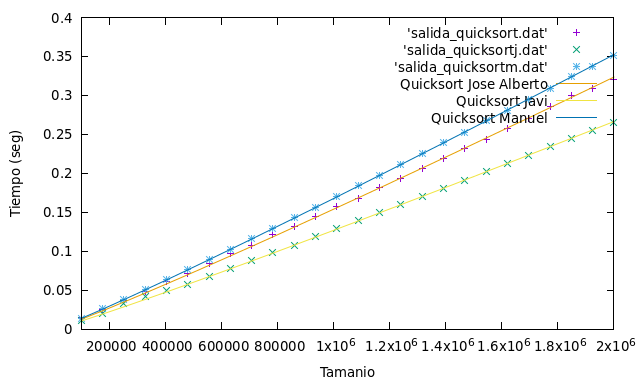
\includegraphics[scale=0.3]{../../Images/Quicksort_combinados.png}
\caption{Gráfica con los tiempos de ejecución del \\algoritmo de Quicksort}
\end{figure}

Tras representar en la gráfica los 26 puntos obtenidos con la ejecución del algoritmo de Quicksort, con gnuplot vemos que las constantes ocultas son:
\begin{itemize}
	\item Ordenador Javier \(\rightarrow T_1(n) = 6.30121 \cdot 10^{-9} x\log(x) + 0.00188054\). 
	\item Ordenador José Alberto \(\rightarrow T_2(n) = 7.62891 \cdot 10^{-9} x\log(x) + 0.00283755\).
	\item Ordenador Manuel \(\rightarrow T_3(n) = 8.39387 \cdot 10^{-9} x\log(x) + 0.000666717\).
\end{itemize} 

Podemos observar que nuestro análisis teórico es correcto. Además, podemos observarlo con el coeficiente de regresión para cada una de nuestra funciones de ajuste:
\begin{itemize}
	\item \(T_1(n) \longrightarrow Var.res = 0.000000796551\)
	\item \(T_2(n) \longrightarrow Var.res = 0.00000158349\)
	\item \(T_3(n) \longrightarrow Var.res = 0.0000000913545\)
\end{itemize}

Como los valores son muy próximos a 0 vemos realmente que el ajuste es bueno.

\subsection{Heapsort}
\lstinputlisting[language=C++]{./Codes/heapsort.cpp}
\subsubsection{Eficiencia teórica}
Observando el código podemos ver como el algoritmo se divide en dos bucles los cuales al no estar anidados cogeremos el tiempo del máximo de los dos. Por tanto es fácil ver como ambos bucles tienen la misma complejidad donde en el peor de los casos se ejecuta n veces y por tanto, al ser la función \texttt{reajustar} de complejidad \(\mathcal{O}(\log(n))\), tenemos que la complejidad del algoritmo es \(\mathcal{O}(n\log(n))\). La función \texttt{reajustar} es \(\mathcal{O}(\log(n))\) porque en cada iteración se ejecuta como máximo la profundidad del árbol que se usa en el algoritmo, siendo dicha profundidad \(\log(n)\). Por tanto tenemos que
\[
T(n) \in \mathcal{O}(n\log(n))
\]
donde \(T(n)\) es la función que expresa el tiempo de ejecución del algoritmo.

\subsubsection{Eficiencia empírica}
Tras ejecutar el algortimo en un rango de 100000 a 2000000 elementos, con saltos de 76000 unidades por ejecución, obtenemos los siguientes resultados:

\begin{table}[h!]
	\centering
	\footnotesize
	\scalebox{0.75}{
		\begin{tabular}{|c|c|}
			\hline
			\multicolumn{2}{|c|}{\textsf{Ordenador Javier}}
			\\\hline
			\bfseries Elementos (n) & \bfseries Tiempo (s)
			\csvreader{./data/Javi5454/salida_heapsort.csv}{}
			{\\\hline\csvcoli&\csvcolii}
			\\\hline
		\end{tabular}
	}
	\hspace{2cm}
	\scalebox{0.75}{
		\begin{tabular}{|c|c|}
			\hline
			\multicolumn{2}{|c|}{\textsf{Ordenador José Alberto}}
			\\\hline
			\bfseries Elementos (n) & \bfseries Tiempo (s)
			\csvreader{./data/Jota/salida_heapsort.csv}{}
			{\\\hline\csvcoli&\csvcolii}
			\\\hline
		\end{tabular}
	}
	\hspace{2cm}
	\scalebox{0.75}{
		\begin{tabular}{|c|c|}
			\hline
			\multicolumn{2}{|c|}{\textsf{Ordenador Manuel}}
			\\\hline
			\bfseries Elementos (n) & \bfseries Tiempo (s)
			\csvreader{./data/Moya/salida_heapsort.csv}{}
			{\\\hline\csvcoli&\csvcolii}
			\\\hline
		\end{tabular}
	}
	\caption{Experiencia empírica de algoritmo de Heapsort}
\end{table}

Se pueden observar pequeñas diferencias entre los distintos tiempos de ejecución pero no muy notables, debidas como hemos comentado anteriormente a las distintas características entre los ordenadores en los que se han ejecutado los programas.

\subsubsection{Eficiencia híbrida}
A continuación comprobaremos como la función de ajuste teórico obtenida es la correcta con la eficiencia híbrida. Tomaremos los datasets de los integrantes del grupo para visualizarlo. \\

\begin{figure}[h!]
\centering
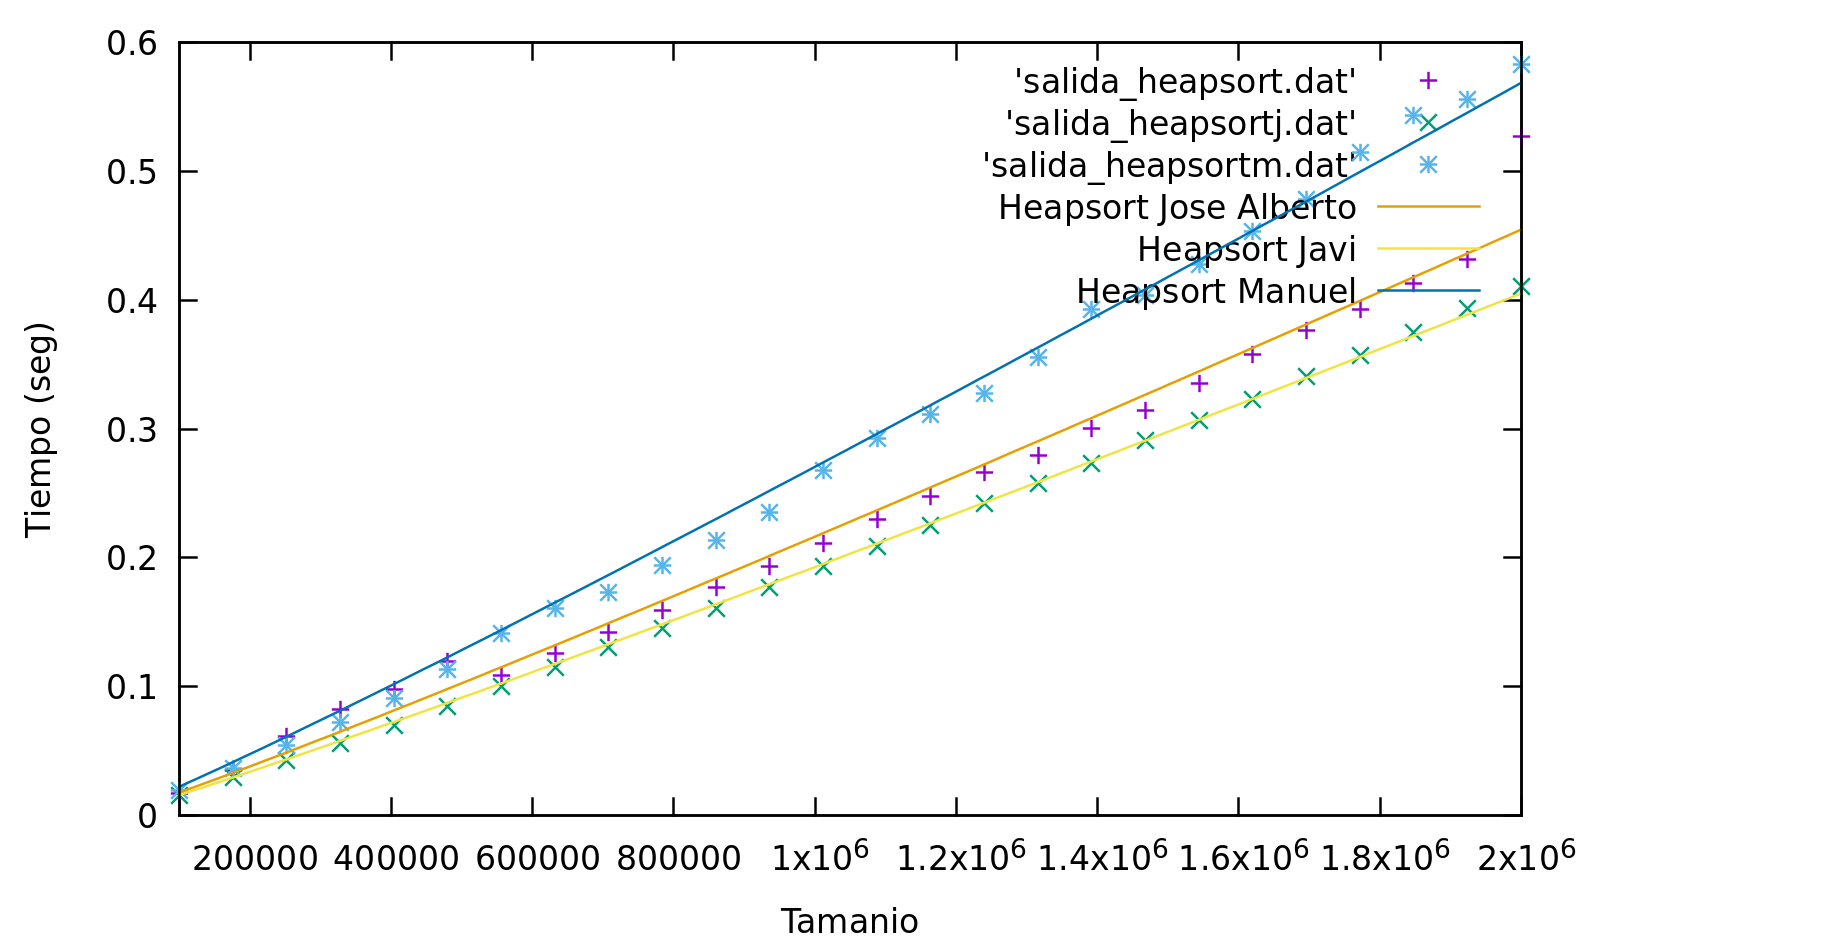
\includegraphics[scale=0.15]{../../Images/Heapsort_combinados.png}
\caption{Gráfica con los tiempos de ejecución del \\algoritmo de Heapsort}
\end{figure}

Tras representar en la gráfica los 26 puntos obtenidos con la ejecución del algoritmo de Heapsort, es fácil calcular con gnuplot que las constantes ocultas son:
\begin{itemize}
	\item Ordenador Javier \(\rightarrow T_1(n) = 9.81428 \cdot 10^{-9} xlog(x) - 0.00367709\). 
	\item Ordenador José Alberto \(\rightarrow T_2(n) = 1.08739 \cdot 10^{-8} xlog(x) - 0.000156439\).
	\item Ordenador Manuel \(\rightarrow T_3(n) = 1.41147 \cdot 10^{-8} xlog(x) - 0.0148078\).
\end{itemize} 

Podemos observar que nuestro análisis teórico es correcto. Además, podemos observarlo con el coeficiente de regresión para cada una de nuestra funciones de ajuste:
\begin{itemize}
	\item \(T_1(n) \longrightarrow Var.res = 0.00265428\)
	\item \(T_2(n) \longrightarrow Var.res = 0.00031452\)
	\item \(T_3(n) \longrightarrow Var.res = 0.000056906\)
\end{itemize}

El ajusto es bueno pues los valores resultantes son próximos a 0.

\subsection{Comparativa de los algoritmos de ordenación}

En este apartado vamos a ver claramente cuál es la diferencia entre los 4 algoritmos de ordenación que acabamos de analizar. Para ello, hemos generado una gráfica conjunta con las funciones de ajuste ya halladas antes, que eran:

\begin{itemize}
	\item Inserción Javier \(\rightarrow T_1(n) = 8.49924 \cdot 10^{-10} x^2 - 8.57879 \cdot 10^{-6} x + 0.546581\).
	\item Selección Javier \(\rightarrow T_1(n) = 1.0371 \cdot 10^{-9} x^2 + -9.86278 \cdot 10^{-6} x +0.0216418\).
	\item Quicksort Javier \(\rightarrow T_1(n) = 9.18701 \cdot 10^{-9} \cdot x \cdot log(x)\).
	\item Heapsort Javier \(\rightarrow T_1(n) = 1.39707 \cdot 10^{-8} \cdot x \cdot log(x)\).
\end{itemize}

\begin{itemize}
	\item Inserción José Alberto \(\rightarrow T_2(n) = 7.96341 \cdot 10^{-10} x^2 + 2.23563 \cdot 10^{-5} x - 0.592279\).
	\item Selección José Alberto \(\rightarrow T_2(n) = 1.17905 \cdot 10^{-9} x^2 + 3.97249 \cdot 10^{-7} x - 0.00421685\).
	\item Quicksort José Alberto \(\rightarrow T_2(n) = 1.11515 \cdot 10^{-8} \cdot x \cdot log(x)\).
	\item Heapsort José Alberto \(\rightarrow T_2(n) = 1.56798 \cdot 10^{-8} \cdot x \cdot log(x)\).
\end{itemize}

\begin{itemize}
	\item Inserción Manuel \(\rightarrow T_3(n) = 1.04394 \cdot 10^{-9} x^2 + 1.58593 \cdot 10^{-6} x - 0.0969414\).
	\item Selección Manuel \(\rightarrow T_3(n) = 1.29484 \cdot 10^{-9} x^2 - 7.43377 \cdot 10^{-6} x + 0.0733569\).
	\item Quicksort Manuel \(\rightarrow T_3(n) = 1.21439 \cdot 10^{-8} \cdot x \cdot log(x)\).
	\item Heapsort Manuel \(\rightarrow T_3(n) = 1.96051 \cdot 10^{-8} \cdot x \cdot log(x)\).
\end{itemize}

\begin{figure}[h!]
	\begin{subfigure}{.5\textwidth}
		\centering
		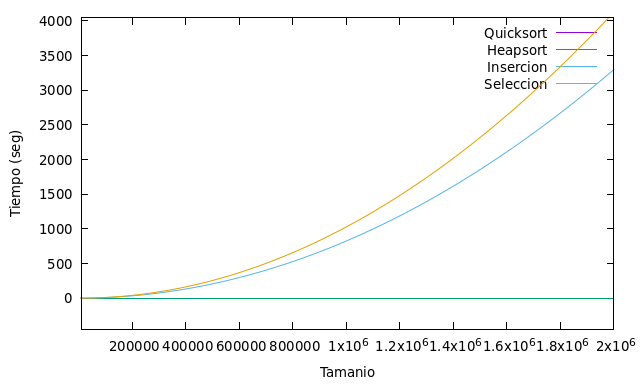
\includegraphics[scale=0.4]{../../Images/Grafica_comparativa_algoritmos_ordenacion_Javi5454.png}
		\caption{Ordenador Javier}
	\end{subfigure}
	\hfill
	\begin{subfigure}{.5\textwidth}
		\centering
		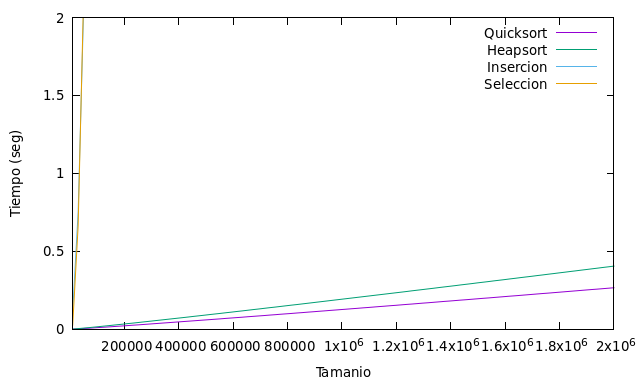
\includegraphics[scale=0.4]{../../Images/Grafica_comparativa_algoritmos_ordenacion_Javi5454_(HyQ).png}
		\caption{Ordenador Javier}
	\end{subfigure}
\end{figure}
 
 \begin{figure}[h!]
 	\begin{subfigure}{.5\textwidth}
 		\centering
 		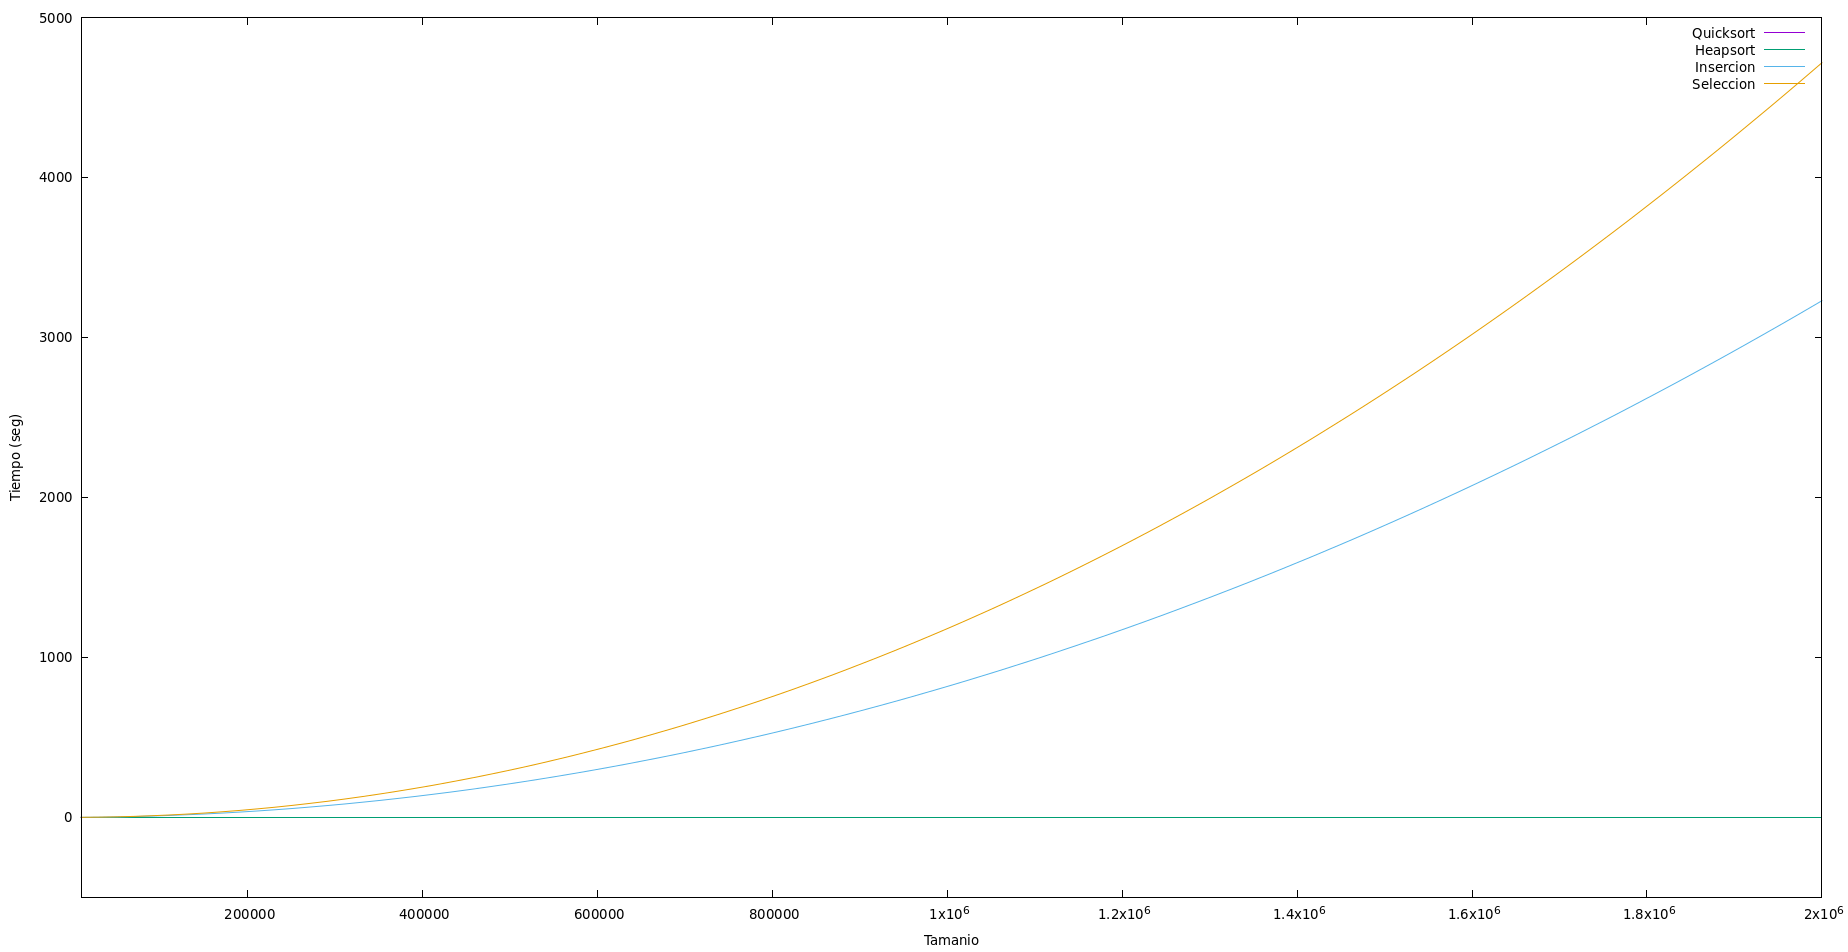
\includegraphics[scale=0.13]{../../Images/Grafica_comparativa_algoritmos_de_ordenacion_Joshoccas.png}
 		\caption{Ordenador José Alberto}
 	\end{subfigure}
 	\hfill
 	\begin{subfigure}{.5\textwidth}
 		\centering
 		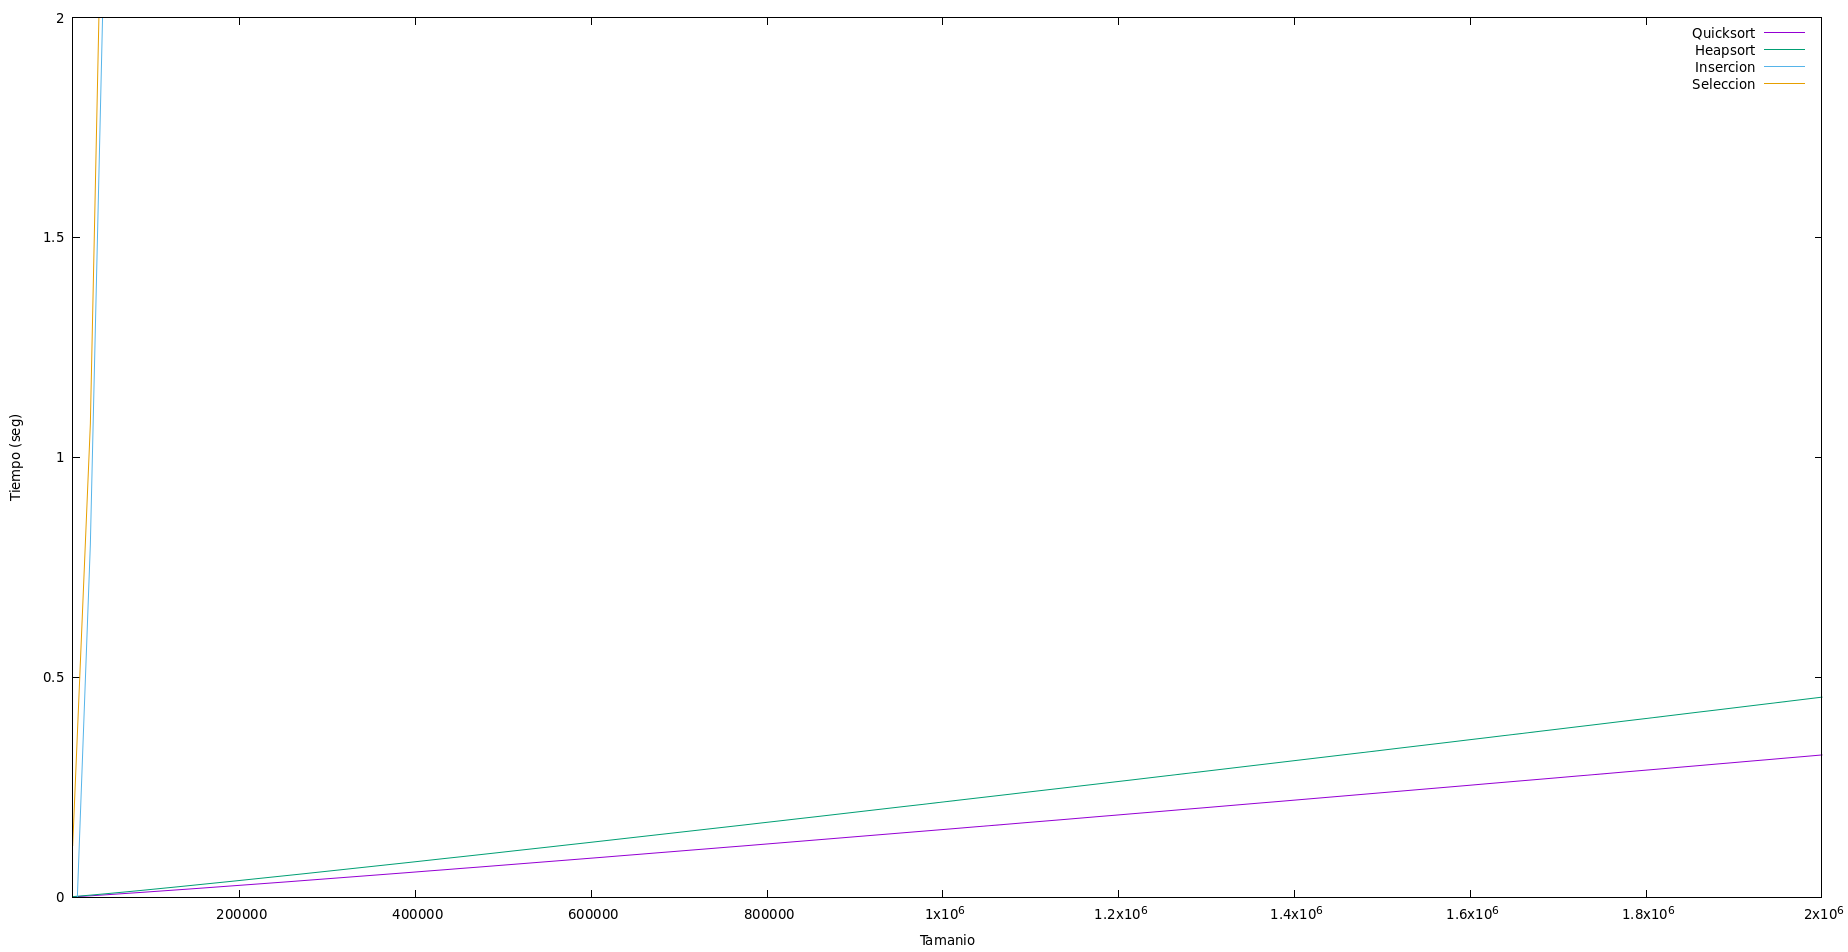
\includegraphics[scale=0.13]{../../Images/Grafica_comparativa_algoritmos_ordenacion_Joshoccas_(HyQ).png}
 		\caption{Ordenador José Alberto}
 	\end{subfigure}
 \end{figure}

\begin{figure}[h!]
	\begin{subfigure}{.5\textwidth}
		\centering
		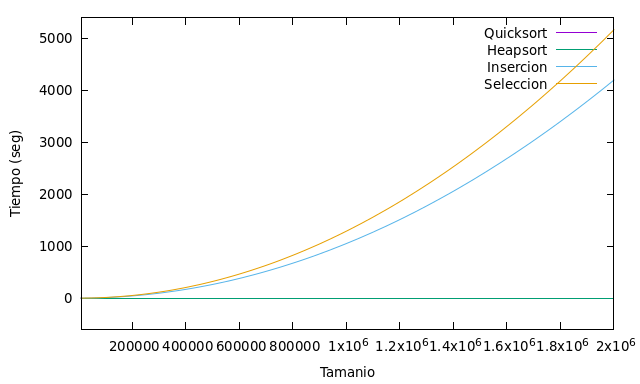
\includegraphics[scale=0.35]{../../Images/Grafica_comparativa_algoritmos_ordenacion_ManuelMoya.png}
		\caption{Ordenador Manuel}
	\end{subfigure}
	\hfill
	\begin{subfigure}{.5\textwidth}
		\centering
		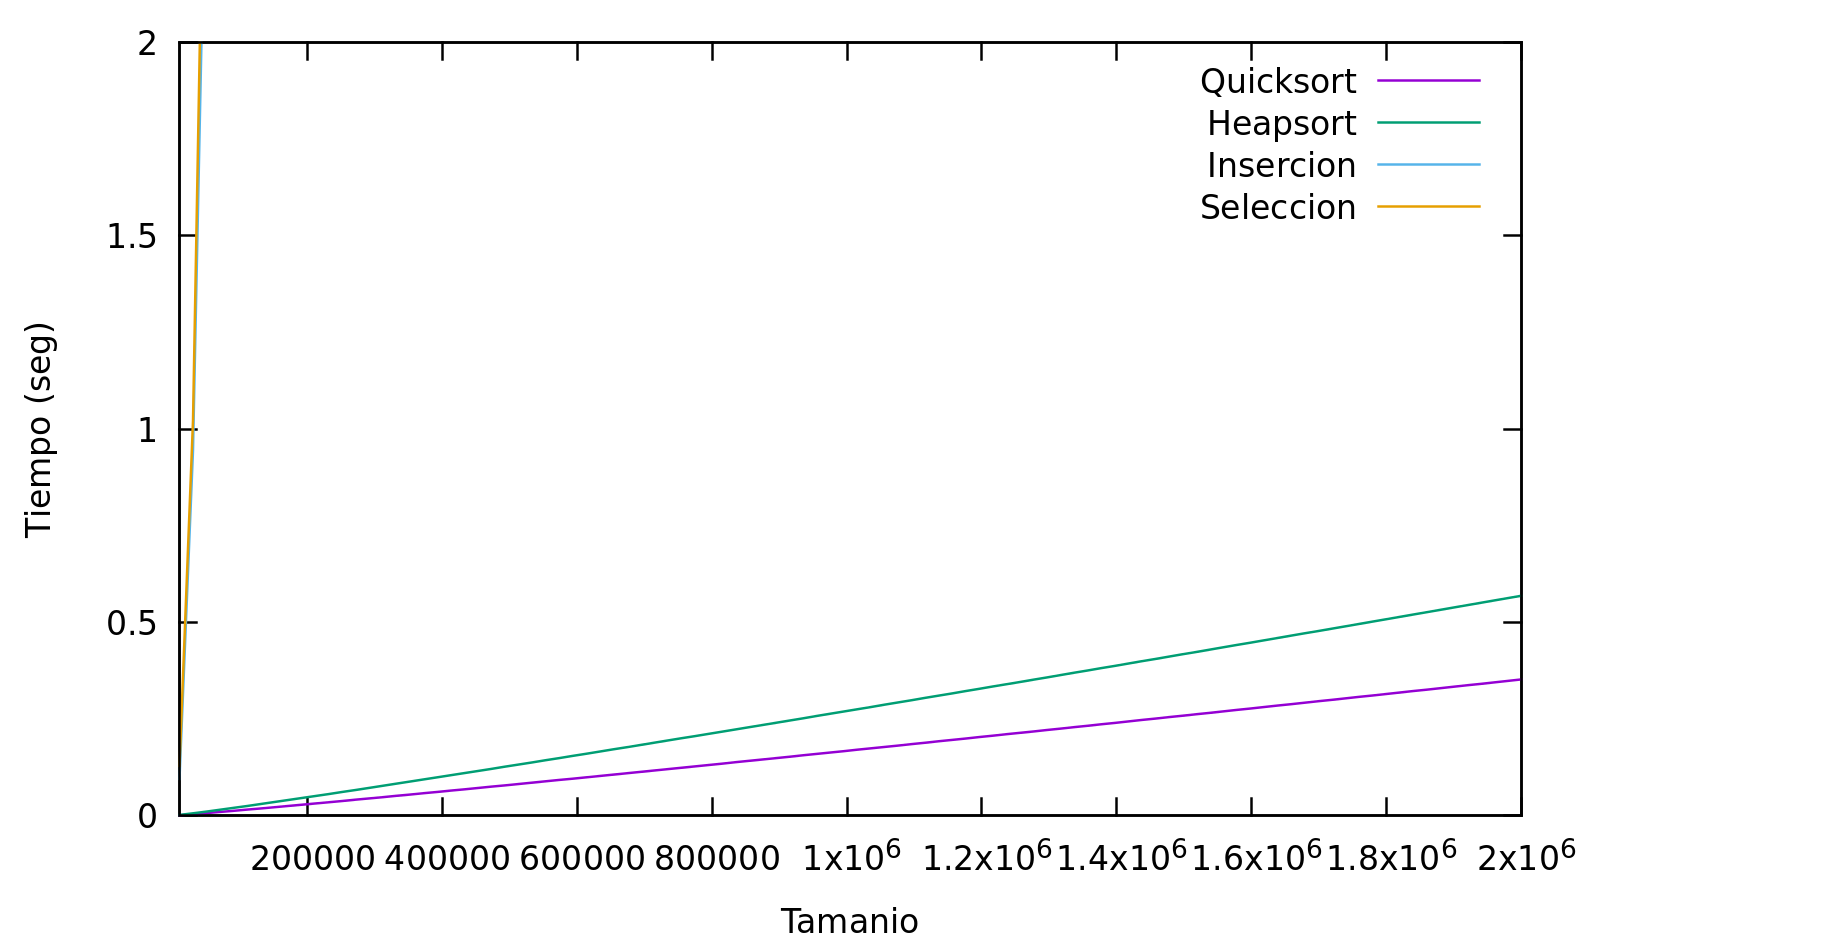
\includegraphics[scale=0.15]{../../Images/Grafica_comparativa_algoritmos_ordenacion_ManuelMoya_(HyQ).png}
		\caption{Ordenador Manuel}
	\end{subfigure}
\end{figure}

Hemos hecho 2 gráficas porque al realizar la primera de cada par correspondiente a cada integrante, vimos que quicksort y heapsort se veían como una línea paralela al eje X en la que no se diferencian entre sí. Esto se debe a la gran diferencia entre los tiempos de estos dos algoritmos con respecto a los que tienen eficiencia cuadrática, que son inserción y selección, los cuales llegan a más de 5000 segundos por ejecución, mientras que los de eficiencia logarítmica no llegan a sobrepasar el segundo por ejecución. Así, en la segunda gráfica restringimos el rango del eje Y de 0 a 2 para que se pudiese ver que realmente quicksort y heapsort sí se diferencian entre ellos y se ve que tienen cierta pendiente, insignificante respecto a la pendiente de inserción y selección. Por lo tanto, una vez más vemos que nuestro análisis tiene sentido y se corresponde con los datasets obtenidos.

\subsection{Floyd}
\lstinputlisting[language=Python]{./Codes/floyd.cpp}

\subsubsection{Eficiencia teórica}

Como podemos observar en los comentarios del código que hemos hecho en la función \texttt{void Floyd}, estamos ante una función que pertenece a \(\mathcal{O}(n^3)\). Son tres bucles \texttt{for} que están anidados, cada uno \(\mathcal{O}(n)\), por tanto, multiplicando los órdenes obtenemos que la función es \(\mathcal{O}(n^3)\), es decir,
\[
	T(n) \in \mathcal{O}(n^3)
\]
donde \(T(n)\) es la función que expresa el tiempo de ejecución del algoritmo.

\subsubsection{Eficiencia empírica}

Tras ejecutar el algoritmo en un rango de 176 a 2000 elementos, con saltos de 76 unidades por ejecución, obtenemos los siguientes resultados:

\begin{table}[h!]
	\centering
	\footnotesize
	\scalebox{0.75}{
		\begin{tabular}{|c|c|}
			\hline
			\multicolumn{2}{|c|}{\textsf{Ordenador Javier}}
			\\\hline
			\bfseries Elementos (n) & \bfseries Tiempo (s)
			\csvreader{./data/Javi5454/salida_floyd.csv}{}
			{\\\hline\csvcoli&\csvcolii}
			\\\hline
		\end{tabular}
		}
		\hspace{2cm}
		\scalebox{0.75}{
		\begin{tabular}{|c|c|}
			\hline
			\multicolumn{2}{|c|}{\textsf{Ordenador José Alberto}}
			\\\hline
			\bfseries Elementos (n) & \bfseries Tiempo (s)
			\csvreader{./data/Jota/salida_floyd.csv}{}
			{\\\hline\csvcoli&\csvcolii}
			\\\hline
			\end{tabular}
			}
		\hspace{2cm}
		\scalebox{0.75}{
		\begin{tabular}{|c|c|}
			\hline
			\multicolumn{2}{|c|}{\textsf{Ordenador Manuel}}
			\\\hline
			\bfseries Elementos (n) & \bfseries Tiempo (s)
			\csvreader{./data/Moya/salida_floyd.csv}{}
			{\\\hline\csvcoli&\csvcolii}
			\\\hline
		\end{tabular}
		}
		\caption{Experiencia empírica de algoritmo de Floyd sin optimizar}
\end{table}

Observamos pequeñas diferencias, pero en general nada fuera de lo común. Estas diferencias son debidas a los distintos agentes tecnológicos usados para la realización del análisis de la eficiencia empírica en esta práctica.

\subsubsection{Eficiencia híbrida}

A través de la eficiencia híbrida, comprobaremos que el ajuste teórico realizado es correcto. Para realizar este análisis, tomamos los datasets de todos los integrantes del grupo. \\

\begin{figure}[h!]
\centering
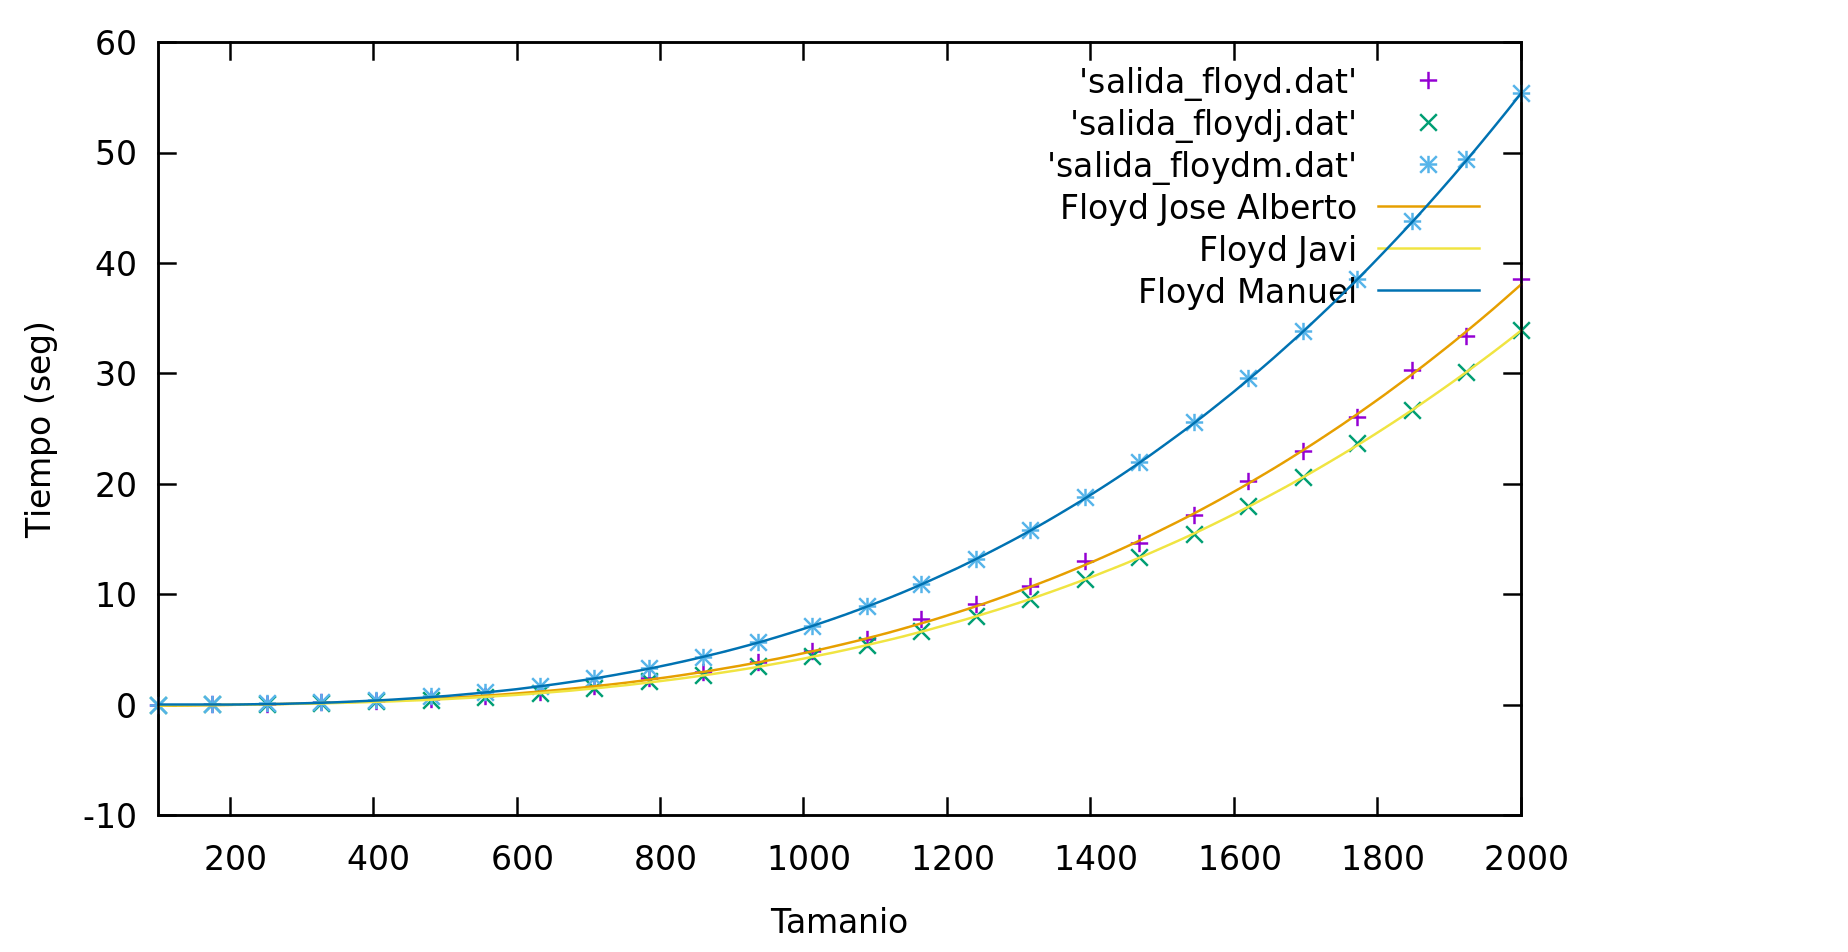
\includegraphics[scale=0.15]{../../Images/floyd_combinados.png}
\caption{Gráfica con los tiempos de ejecución del \\algoritmo de Floyd}
\end{figure}

\newpage

En esta gráfica están representados los 26 puntos obtenidos tras la ejecución del algoritmo de Floyd en los distintos equipos de los integrantes del grupo. Tras una serie de cálculos con gnuplot, observamos que las constantes ocultas son:
\begin{itemize}
	\item Ordenador Javier \(\rightarrow T_1(n) = 4.38237 \cdot 10^{-9} x^3 -4.33753 \cdot 10^{-7} x^2 + 0.000337001 x -0.0504332\).
	\item Ordenador José Alberto \(\rightarrow T_2(n) = 5.12922 \cdot 10^{-9} x^3 -1.11315 \cdot 10^{-6} x^2 + 0.00083571 x - 0.134397\).
	\item Ordenador Manuel \(\rightarrow T_3(n) = 6.77297 \cdot 10^{-9} x^3 + 5.13099 \cdot 10^{-7} x^2 - 0.000427834 x + 0.0714028\).
\end{itemize} 

Podemos observar que nuestro análisis teórico es correcto. Además, podemos observarlo con el coeficiente de regresión para cada una de nuestra funciones de ajuste:
\begin{itemize}
	\item \(T_1(n) \longrightarrow Var.res = 0.00204522\)
	\item \(T_2(n) \longrightarrow Var.res = 0.044778\)
	\item \(T_3(n) \longrightarrow Var.res = 0.000855184\)
\end{itemize}

Estos valores son muy cercanos a 0, y por tanto indican que el ajuste es muy bueno.
\subsection{Hanoi}
\lstinputlisting[language=C++]{./Codes/hanoi.cpp}

\subsubsection{Eficiencia teórica}

En este caso no podemos realizar un análisis de la misma manera que en el algoritmo anterior, pues estamos ante un algoritmo recursivo. De esta manera, trataremos de buscar la relación de recurrencia.

Suponiendo que estamos en la \(n\)-ésima iteración, el algoritmo comprobará lo indicado en el \texttt{if}, que es de \(\mathcal{O}(1)\), y volverá a llamarse a sí misma otras dos veces. Por tanto, la ecuación de recurrencia es la siguiente:
\[
	T_n = 2T_{n-1} + 1
\]

Si resolvemos la ecuación de recurrencia obtenemos que:
\[
	(x-2)(x-1) = 0
\]
\[
	t_n = c_1 \cdot 2^n + c_2
\]

Y concluimos que \(T(n) \in \mathcal{O}(2^n)\), donde \(T(n)\) es la función que expresa el tiempo de ejecución de nuestro algortimo para \(n\) elementos.

\newpage

\subsubsection{Eficiencia empírica}
Debido al orden del algoritmo, el número de elementos que tenemos que tomar es mucho menor que los que usamos en el resto de algortimos. En este caso, tras ejecutar el algoritmo en un rango de 7 a 32 elementos, con saltos de 1 elemento por iteración, obtenemos los siguientes resultados:

\begin{table}[h!]
	\centering
	\footnotesize
	\scalebox{0.75}{
		\begin{tabular}{|c|c|}
			\hline
			\multicolumn{2}{|c|}{\textsf{Ordenador Javier}}
			\\\hline
			\bfseries Elementos (n) & \bfseries Tiempo (s)
			\csvreader{./data/Javi5454/salida_hanoi.csv}{}
			{\\\hline\csvcoli&\csvcolii}
			\\\hline
		\end{tabular}
		}
		\hspace{2cm}
		\scalebox{0.75}{
		\begin{tabular}{|c|c|}
			\hline
			\multicolumn{2}{|c|}{\textsf{Ordenador José Alberto}}
			\\\hline
			\bfseries Elementos (n) & \bfseries Tiempo (s)
			\csvreader{./data/Jota/salida_hanoi.csv}{}
			{\\\hline\csvcoli&\csvcolii}
			\\\hline
			\end{tabular}
			}
		\hspace{2cm}
		\scalebox{0.75}{
		\begin{tabular}{|c|c|}
			\hline
			\multicolumn{2}{|c|}{\textsf{Ordenador Manuel}}
			\\\hline
			\bfseries Elementos (n) & \bfseries Tiempo (s)
			\csvreader{./data/Moya/salida_hanoi.csv}{}
			{\\\hline\csvcoli&\csvcolii}
			\\\hline
		\end{tabular}
		}
		\caption{Experiencia empírica de algoritmo de Hanoi}
\end{table}

Aquí si que observamos grandes diferencias entre los dos primeros equipos y el tercero. Esto puede ser debido a el procesador de estos, o el hecho de que el tercer equipo es un portátil y la ejecución del programa se realizó sin cargar el equipo. Esto en ocasiones puede provocar bajada de rendimiento.

\subsubsection{Eficiencia híbrida}

Este análisis confirmará nuestro análisis teórico. Para realizar este análisis, tomamos los datasets de todos los integrantes del grupo.

\begin{figure}[h!]
\centering
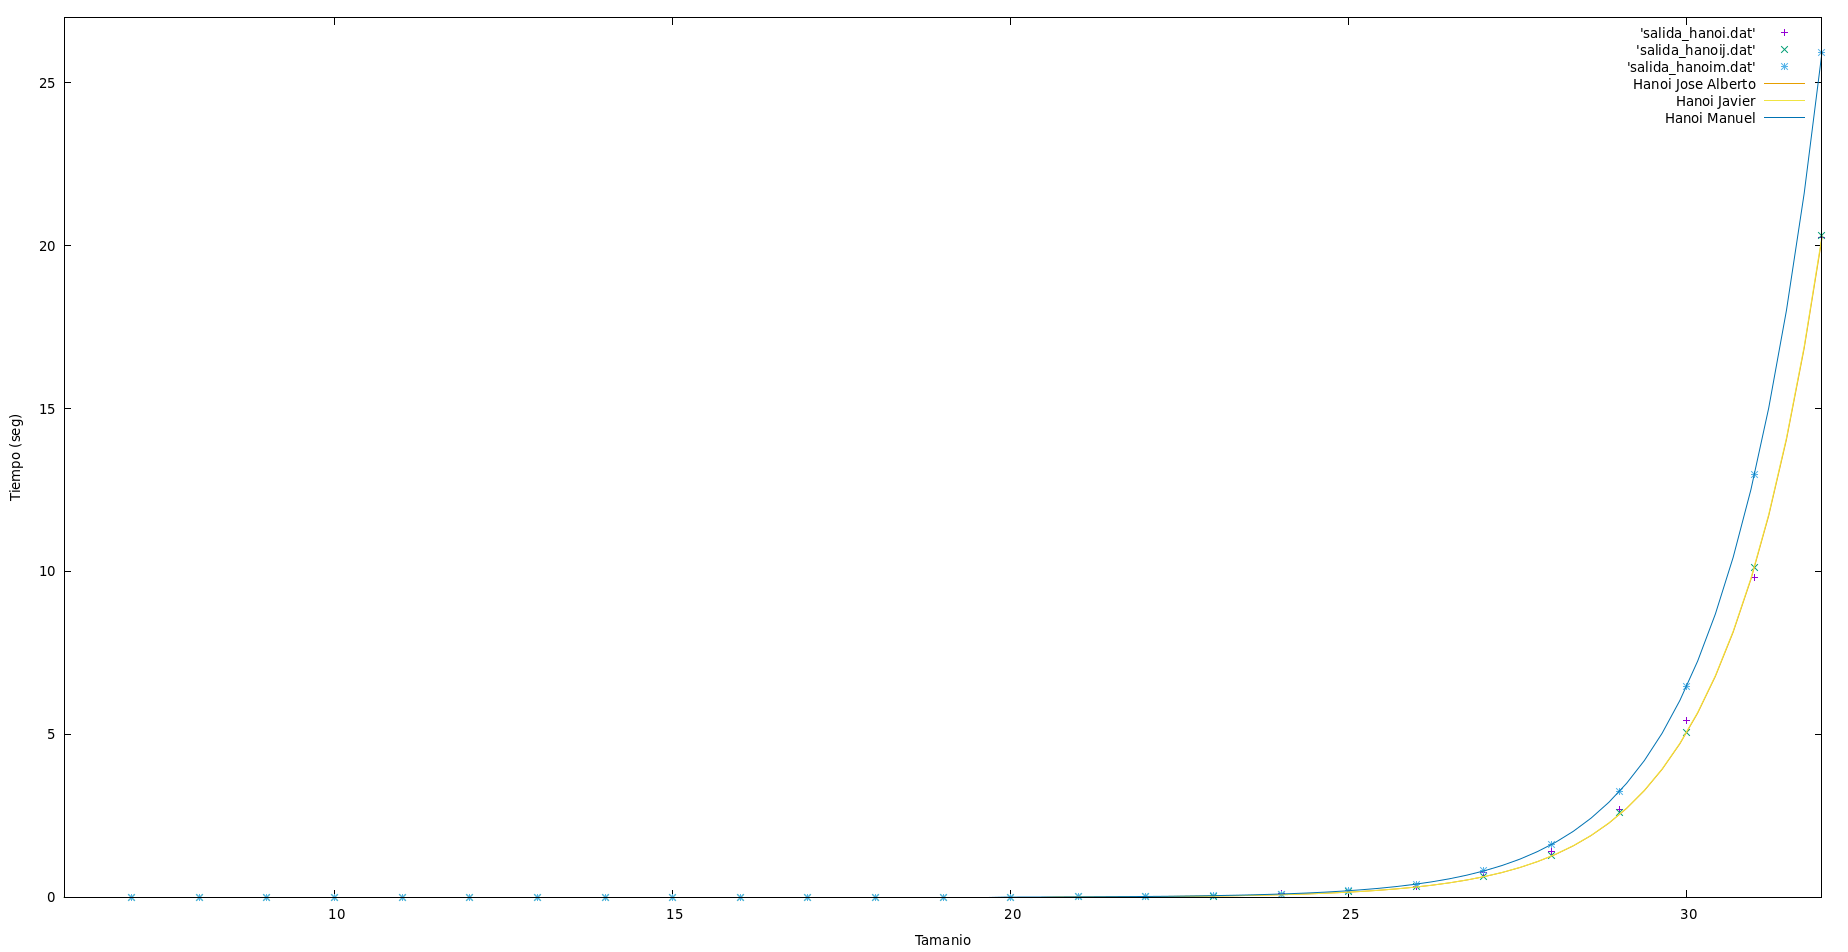
\includegraphics[scale=0.17]{../../Images/hanoi_combinados.png}
\caption{Gráfica con los tiempos de ejecución del \\algoritmo de las torres de Hanoi}
\end{figure}

\newpage

En esta gráfica están representados los 26 puntos obtenidos tras la ejecución del algoritmo de Hanoi en los distintos equipos de los integrantes del grupo. Tras una serie de cálculos con gnuplot, observamos que las constantes ocultas son:
\begin{itemize}
	\item Ordenador Javier \(\rightarrow T_1(n) = 4.72408 \cdot 10^{-9} \cdot 2^x\).
	\item Ordenador José Alberto \(\rightarrow T_2(n) = 4.70707 \cdot 10^{-9} \cdot 2^x\).
	\item Ordenador Manuel \(\rightarrow T_3(n) = 6.03512 \cdot 10^{-9} \cdot 2^x\).
\end{itemize}

Podemos observar que nuestro análisis teórico es correcto. Además, podemos observarlo con el coeficiente de regresión para cada una de nuestras funciones de ajuste:
\begin{itemize}
	\item \(T_1(n) \longrightarrow Var.res = 0.000302074\)
	\item \(T_2(n) \longrightarrow Var.res = 0.0113386\)
	\item \(T_3(n) \longrightarrow Var.res = 3.87795 \cdot 10^{-7}\)
\end{itemize}

Estos valores son muy cercanos a 0, y por tanto indican que el ajuste es muy bueno.

\section{Casos especiales}

Además del análisis mostrado de los seis algoritmos anteriores, también se ha realizado un análisis de algunos de ellos bajo condiciones distintas, para mostrar así además una experiencia más amplia y diversa y conseguir un mejor entendimiento de los algortimos trabajados.

\subsection{Floyd optimizado}

En este caso, queríamos mostrar la diferencia que obtenemos cuando realizamos la compilación de nuestro código bajo ciertas condiciones que pueden modificar "la pureza del mismo". 

Con una compilación normal, el compilador tratará de convertir nuestros \texttt{.cpp} a código máquina de la manera más fiel posible. Sin embargo, si la introducimos la orden \texttt{-Og} estamos indicando a este que reduzca en lo máximo la ineficiencia de nuestro código, optimizándolo.

A continuación, se muestra una comparación de tiempos de ejecución:

\begin{table}[h!]
	\centering
	\footnotesize
	\scalebox{0.75}{
		\begin{tabular}{|c|c|}
			\hline
			\multicolumn{2}{|c|}{\textsf{Ordenador Javier}}
			\\\hline
			\bfseries T. Sin optimizar (s) & \bfseries T. Optimizado (s)
			\csvreader{./data/Javi5454/salida_floyd_optimizado.csv}{}
			{\\\hline\csvcoli&\csvcolii}
			\\\hline
		\end{tabular}
		}
		\hspace{2cm}
		\scalebox{0.75}{
		\begin{tabular}{|c|c|}
			\hline
			\multicolumn{2}{|c|}{\textsf{Ordenador José Alberto}}
			\\\hline
			\bfseries T. Sin optimizar (s) & \bfseries T. Optimizado (s)
			\csvreader{./data/Jota/salida_floyd_optimizado.csv}{}
			{\\\hline\csvcoli&\csvcolii}
			\\\hline
			\end{tabular}
			}
		\hspace{2cm}
		\scalebox{0.75}{
		\begin{tabular}{|c|c|}
			\hline
			\multicolumn{2}{|c|}{\textsf{Ordenador Manuel}}
			\\\hline
			\bfseries T. Sin optimizar (s) & \bfseries T. Optimizado (s)
			\csvreader{./data/Moya/salida_floyd_optimizado.csv}{}
			{\\\hline\csvcoli&\csvcolii}
			\\\hline
		\end{tabular}
		}
		\caption{Comparación optimización Floyd}
\end{table}

\begin{figure}[h!]
\begin{subfigure}{.4\textwidth}
	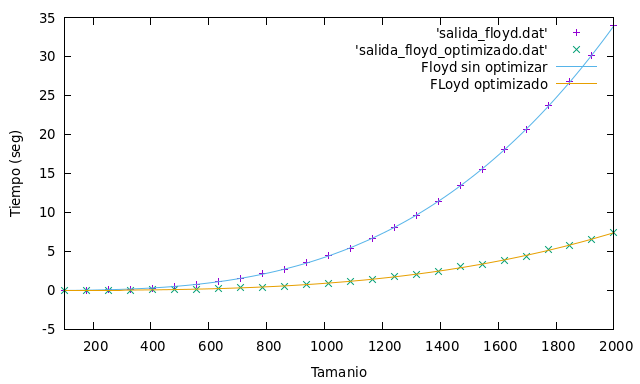
\includegraphics[scale=0.3]{../../Images/floyd_opt_Javi5454.png}
	\caption{Ordenador Javier}
	\label{Floyd Optimizado Javi5454}
\end{subfigure}
\hfill
\begin{subfigure}{.4\textwidth}
	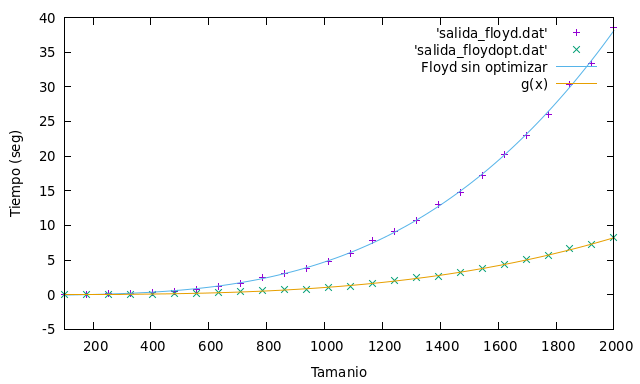
\includegraphics[scale=0.3]{../../Images/floyd_opt_Jota.png}
	\caption{Ordenador José Alberto}
	\label{Floyd Optimizado Jota}
\end{subfigure}
\end{figure}

\begin{figure}[h!]
\centering
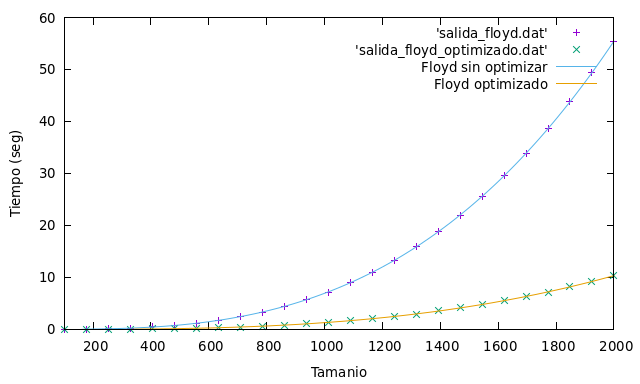
\includegraphics[scale=0.28]{../../Images/floyd_opt_ManuelMoya.png}
\caption*{(c) Ordenador Manuel}
\end{figure}

\newpage

Podemos observar que el uso de la instrucción \texttt{-Og}, y todas sus variantes de su optimización, reducen considerablemente el tiempo de ejecución de nuestro código. Por tanto, su uso debe estar presente a la hora de compilar ciertos programas.

\subsection{Otros posibles ajustes funcionales}

A continuación, se muestran dos gráficas donde se observan otras posibilidades de ajuste para los algoritmos de Floyd y Hanoi, y se observa que los ajustes utilizados en los análisis previos son los mejores, confirmando nuestro análisis teórico.

\begin{figure}[h!]
\begin{subfigure}{.5\textwidth}
	\centering
	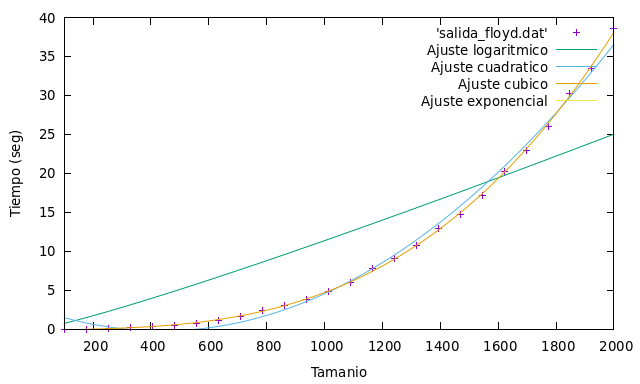
\includegraphics[scale=0.25]{../../Images/floy_comparacion.png}
	\caption{Algoritmo de Floyd}
\end{subfigure}
\begin{subfigure}{.5\textwidth}
	\centering
	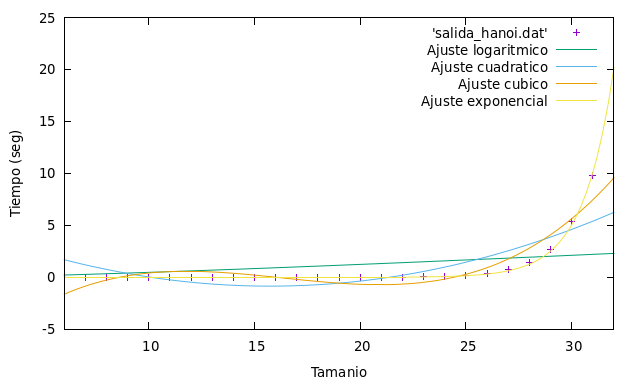
\includegraphics[scale=0.25]{../../Images/hanoi_comparacion.png}
	\caption{Algoritmo de Hanoi}
\end{subfigure}
\end{figure}

Vemos que los órdenes que habíamos obtenido en nuestro análisis teórico son los que mejor se ajustan a nuestra nube de puntos, siendo esto una confirmación de la bondad de nuestro análisis.

\section{Casos en la ejecución de inserción y selección: mejor, peor y promedio}

Otra de las tareas a realizar en esta práctica ha sido medir los tiempos para el mejor caso y peor caso de los algoritmos de inserción y selección y compararlos con el promedio, el cual ya hemos analizado anteriormente. El peor caso es el de un vector ordenado a la inversa, para lo cual hemos introducido en los códigos de inserción y selección el siguiente bucle:

\lstinputlisting[language=Python]{./Codes/peor.cpp}

Y para el mejor caso hemos introducido un bucle que crea un vector ya ordenado:

\lstinputlisting[language=C++]{./Codes/mejor.cpp}

A continuación comenzamos mostrando los datasets del peor y mejor caso de selección y peor y mejor caso de inserción, junto a su representación gráfica:

\begin{table}[h!]
	\centering
	\footnotesize
	\scalebox{0.75}{
		\begin{tabular}{|c|c|}
			\hline
			\multicolumn{2}{|c|}{\textsf{Ordenador Javier}}
			\\\hline
			\bfseries Elementos (n) & \bfseries Tiempo (s)
			\csvreader{./data/Javi5454/salida_seleccion_peor.csv}{}
			{\\\hline\csvcoli&\csvcolii}
			\\\hline
		\end{tabular}
	}
	\hspace{2cm}
	\scalebox{0.75}{
		\begin{tabular}{|c|c|}
			\hline
			\multicolumn{2}{|c|}{\textsf{Ordenador José Alberto}}
			\\\hline
			\bfseries Elementos (n) & \bfseries Tiempo (s)
			\csvreader{./data/Jota/salida_seleccion_peor.csv}{}
			{\\\hline\csvcoli&\csvcolii}
			\\\hline
		\end{tabular}
	}
	\hspace{2cm}
	\scalebox{0.75}{
		\begin{tabular}{|c|c|}
			\hline
			\multicolumn{2}{|c|}{\textsf{Ordenador Moya}}
			\\\hline
			\bfseries Elementos (n) & \bfseries Tiempo (s)
			\csvreader{./data/Moya/salida_seleccion_peor.csv}{}
			{\\\hline\csvcoli&\csvcolii}
			\\\hline
		\end{tabular}
	}
	\caption{Datasets de la ejecución del peor caso para Selección}
\end{table}

\begin{table}[h!]
	\centering
	\footnotesize
	\scalebox{0.75}{
		\begin{tabular}{|c|c|}
			\hline
			\multicolumn{2}{|c|}{\textsf{Ordenador Javier}}
			\\\hline
			\bfseries Elementos (n) & \bfseries Tiempo (s)
			\csvreader{./data/Javi5454/salida_seleccion_mejor.csv}{}
			{\\\hline\csvcoli&\csvcolii}
			\\\hline
		\end{tabular}
	}
	\hspace{2cm}
	\scalebox{0.75}{
		\begin{tabular}{|c|c|}
			\hline
			\multicolumn{2}{|c|}{\textsf{Ordenador José Alberto}}
			\\\hline
			\bfseries Elementos (n) & \bfseries Tiempo (s)
			\csvreader{./data/Jota/salida_seleccion_mejor.csv}{}
			{\\\hline\csvcoli&\csvcolii}
			\\\hline
		\end{tabular}
	}
	\hspace{2cm}
	\scalebox{0.75}{
		\begin{tabular}{|c|c|}
			\hline
			\multicolumn{2}{|c|}{\textsf{Ordenador Moya}}
			\\\hline
			\bfseries Elementos (n) & \bfseries Tiempo (s)
			\csvreader{./data/Moya/salida_seleccion_mejor.csv}{}
			{\\\hline\csvcoli&\csvcolii}
			\\\hline
		\end{tabular}
	}
	\caption{Datasets de la ejecución del mejor caso para Selección}
\end{table}

\begin{table}[h!]
	\centering
	\footnotesize
	\scalebox{0.75}{
		\begin{tabular}{|c|c|}
			\hline
			\multicolumn{2}{|c|}{\textsf{Ordenador Javier}}
			\\\hline
			\bfseries Elementos (n) & \bfseries Tiempo (s)
			\csvreader{./data/Javi5454/salida_insercion_peor.csv}{}
			{\\\hline\csvcoli&\csvcolii}
			\\\hline
		\end{tabular}
	}
	\hspace{2cm}
	\scalebox{0.75}{
		\begin{tabular}{|c|c|}
			\hline
			\multicolumn{2}{|c|}{\textsf{Ordenador José Alberto}}
			\\\hline
			\bfseries Elementos (n) & \bfseries Tiempo (s)
			\csvreader{./data/Jota/salida_insercion_peor.csv}{}
			{\\\hline\csvcoli&\csvcolii}
			\\\hline
		\end{tabular}
	}
	\hspace{2cm}
	\scalebox{0.75}{
		\begin{tabular}{|c|c|}
			\hline
			\multicolumn{2}{|c|}{\textsf{Ordenador Moya}}
			\\\hline
			\bfseries Elementos (n) & \bfseries Tiempo (s)
			\csvreader{./data/Moya/salida_insercion_peor.csv}{}
			{\\\hline\csvcoli&\csvcolii}
			\\\hline
		\end{tabular}
	}
	\caption{Datasets de la ejecución del peor caso para Inserción}
	
\end{table}

\begin{table}[h!]
	\centering
	\footnotesize
	\scalebox{0.7}{
		\begin{tabular}{|c|c|}
			\hline
			\multicolumn{2}{|c|}{\textsf{Ordenador Javier}}
			\\\hline
			\bfseries Elementos (n) & \bfseries Tiempo (s)
			\csvreader{./data/Javi5454/salida_insercion_mejor.csv}{}
			{\\\hline\csvcoli&\csvcolii}
			\\\hline
		\end{tabular}
	}
	\hspace{2cm}
	\scalebox{0.7}{
		\begin{tabular}{|c|c|}
			\hline
			\multicolumn{2}{|c|}{\textsf{Ordenador José Alberto}}
			\\\hline
			\bfseries Elementos (n) & \bfseries Tiempo (s)
			\csvreader{./data/Jota/salida_insercion_mejor.csv}{}
			{\\\hline\csvcoli&\csvcolii}
			\\\hline
		\end{tabular}
	}
	\hspace{2cm}
	\scalebox{0.7}{
		\begin{tabular}{|c|c|}
			\hline
			\multicolumn{2}{|c|}{\textsf{Ordenador Moya}}
			\\\hline
			\bfseries Elementos (n) & \bfseries Tiempo (s)
			\csvreader{./data/Moya/salida_insercion_mejor.csv}{}
			{\\\hline\csvcoli&\csvcolii}
			\\\hline
		\end{tabular}
	}
	\caption{Datasets de la ejecución del mejor caso para Inserción}
	
\end{table}

\newpage

\begin{figure}[h!]
	\begin{subfigure}{.5\textwidth}
		\centering
		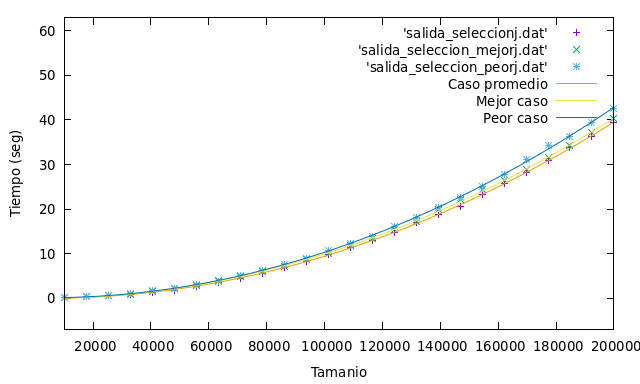
\includegraphics[scale=0.3]{../../Images/Grafica_casos_seleccion_Javi5454.png}
		\caption{Selección Javier}
	\end{subfigure}
	\hfill
	\begin{subfigure}{.5\textwidth}
		\centering
		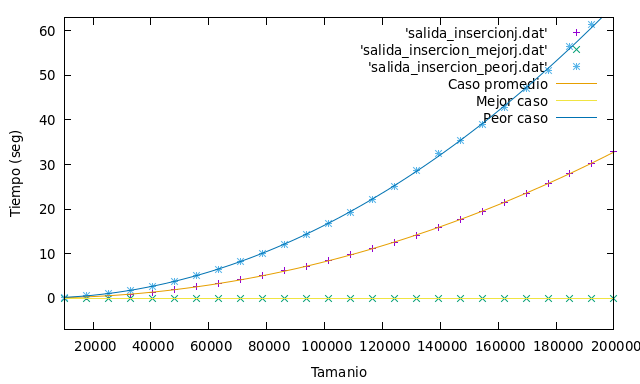
\includegraphics[scale=0.3]{../../Images/Grafica_insercion_casos_Javi5454.png}
		\caption{Inserción Javier}
	\end{subfigure}
\end{figure}

\begin{figure}[h!]
	\begin{subfigure}{.5\textwidth}
		\centering
		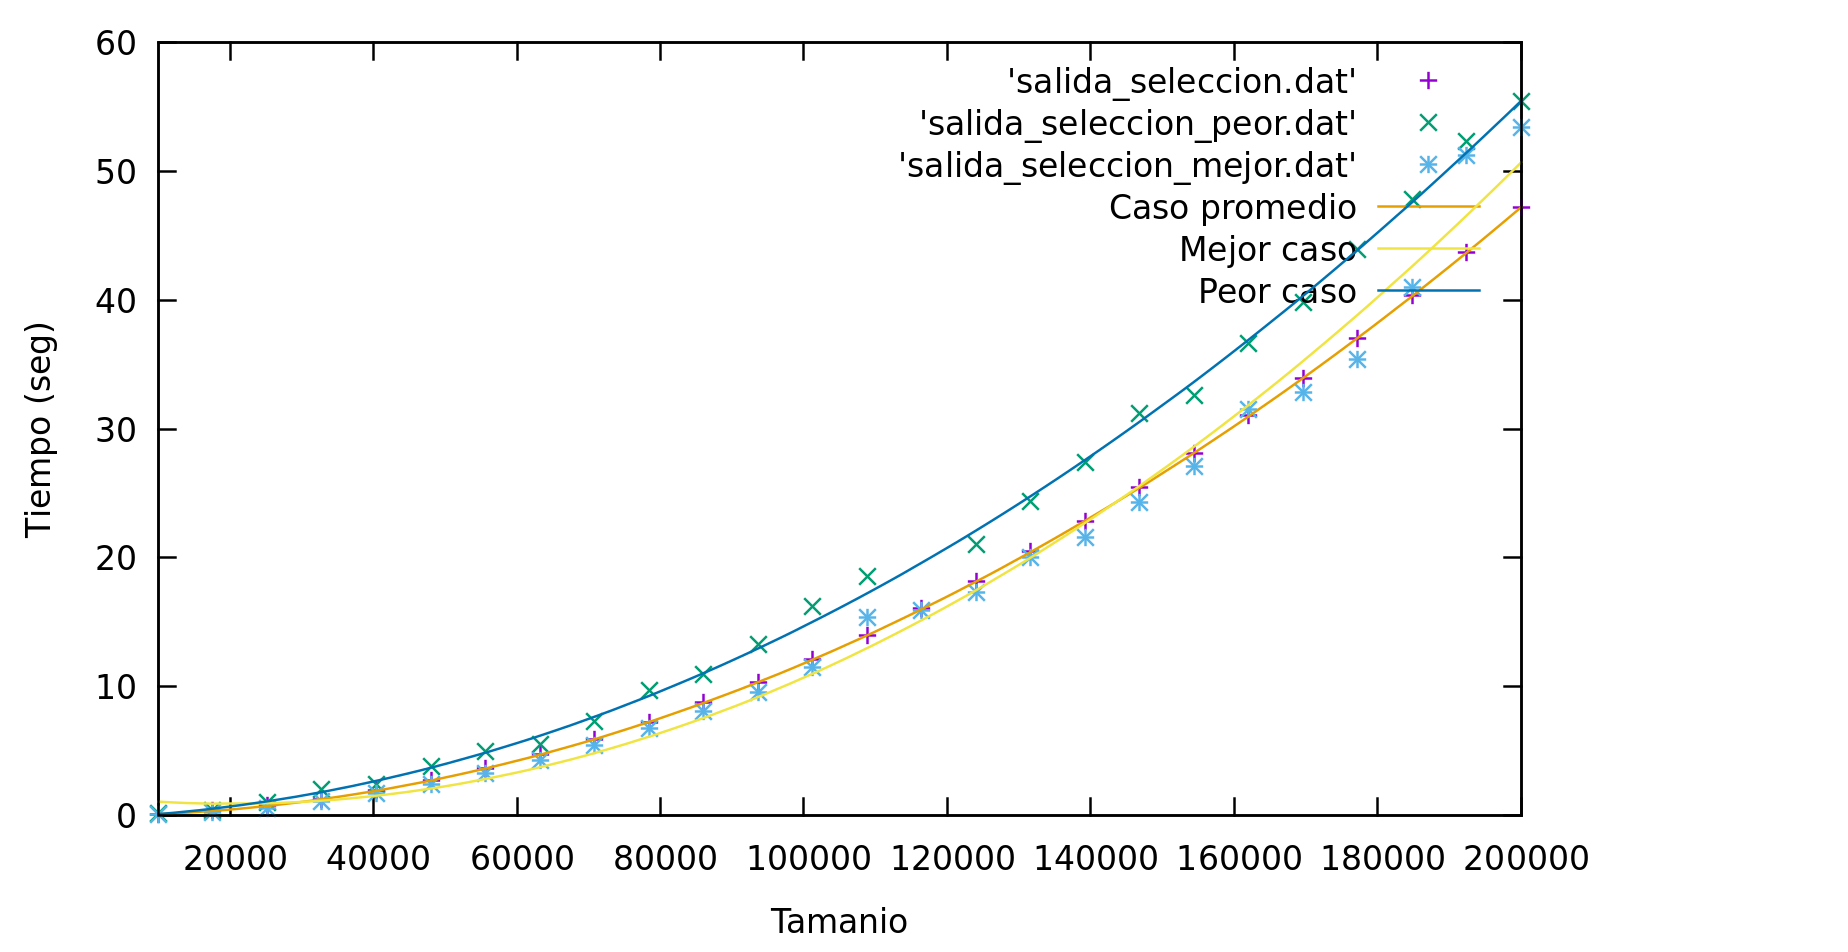
\includegraphics[scale=0.12]{../../Images/Grafica_casos_seleccion_Joshoccas.png}
		\caption{Selección José Alberto}
	\end{subfigure}
	\hfill
	\begin{subfigure}{.5\textwidth}
		\centering
		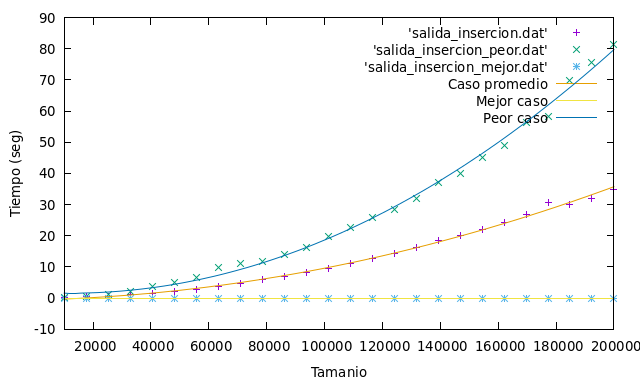
\includegraphics[scale=0.3]{../../Images/Grafica_casos_insercion_Joshoccas.png}
		\caption{Inserción José Alberto}
	\end{subfigure}
\end{figure}

\begin{figure}[h!]
	\begin{subfigure}{.5\textwidth}
		\centering
		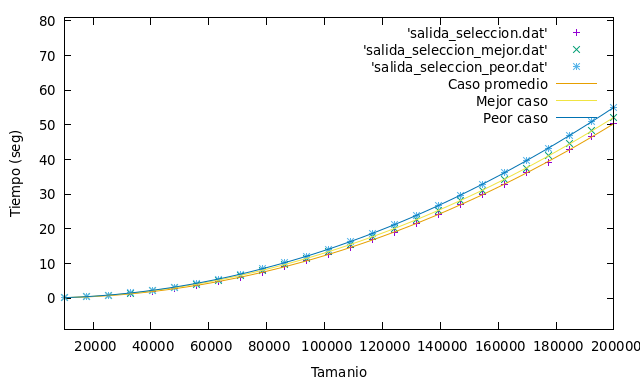
\includegraphics[scale=0.3]{../../Images/Casos_seleccion_ManuelMoya.png}
		\caption{Selección Manuel}
	\end{subfigure}
	\hfill
	\begin{subfigure}{.5\textwidth}
		\centering
		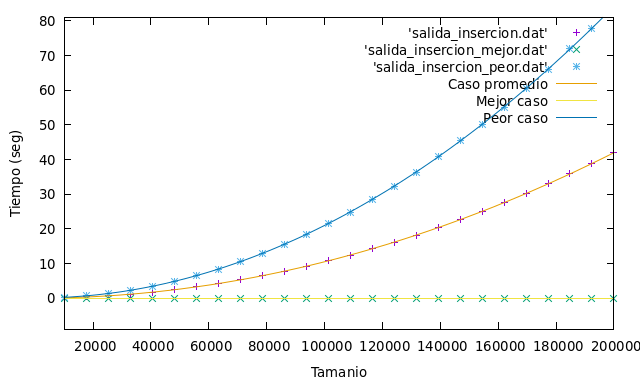
\includegraphics[scale=0.3]{../../Images/Casos_insercion_ManuelMoya.png}
		\caption{Inserción Manuel}
	\end{subfigure}
\end{figure}


\newpage


Como hemos apreciado en las gráficas, en inserción los casos se diferencian perfectamente, tardando casi 0 segundos para el mejor caso y tardando mucho más para el peor caso. Sin embargo, en el algoritmo de selección vemos que las gráficas oscilan en torno a los mismos valores. Esto se debe a cómo están hechos los códigos. En el algoritmo de selección, se comienza hallando el mínimo de los n elementos y se coloca en la primera posición. Tras esto, se calcula el mínimo de los n-1 elementos restantes que no están ordenados y se coloca en segunda posición, y así sucesivamente hasta llegar al final. Por ello, independientemente de que el vector esté ordenado o no, siempre va a tener que recorrer el vector de la forma descrita para hallar todos los mínimos, de ahí que los tiempos en los 3 casos no se diferencien mucho.\\

Por otra parte, en inserción sí se diferencian, y esto se debe a que se ordena de una forma concreta. Este algoritmo ordena "subconjuntos" del vector empezando con los dos primeros elementos. Una vez ordena los dos primeros, inserta el tercero en la posición correcta de entre estos dos. En la siguiente iteración, añade el cuarto elemento a los tres ya ordenados y así sucesivamente hasta acabar. La razón principal de por qué tarda tanto cuando está ordenado es porque cada vez que se va a añadir un elemento a los ya ordenados, se comienza comparando con el último de los ya ordenados, es decir, el mayor de todos (esta comprobación se realiza en el bucle \texttt{while} que se encuentra dentro de un \texttt{for}):

\lstinputlisting[language=C++]{./Codes/insercion.cpp}

De esta forma, como el vector ya está ordenado, la condición del bucle \texttt{while} nunca se da y por lo tanto en cada iteración del \texttt{for} se ahorra la ejecución del cuerpo del bucle \texttt{while} y solo se realizan comparaciones entre pares de números consecutivos.

\newpage

\section{Conclusiones}

Como conclusiones de esta práctica, hemos observado los siguientes hechos a destacar:
\begin{itemize}
	\item El orden de eficiencia de un algoritmo \(\mathcal{O}\) es un factor clave cuando el número de iteraciones a realizar es grande.
	\item Usar optimización a la hora de compilar nuestros programas debe de ser un factor a tener en cuenta, pues puede suponernos una gran ventaja en lo relativo al tiempo de ejecución.
	\item El análisis teórico es importante, pues puede darnos información sobre si merece la pena implementar un algoritmo o no.
	\item El análisis híbrido y la obtención de las constantes ocultas son una manera de confirmar nuestros análisis teórico.
\end{itemize}
\end{document}